\section{Results}\label{sec:results}
Remark: all the time-responses of the nonlinear Rössler system are presented subtracting the operation point, in order to see the references and stabilization easily.
\subsection{Discrete PID Controller}
\subsubsection{Tuning by Reaction Curve}
As described in section \ref{sec:tuning}, the tuning of a PID controller can be performed through the reaction curve. For obtaining the reaction curve, the linearized Rössler system (equation \ref{eq:LinearizedModel}) was simulated for $50s$ using $4^{th}$-order Runge-Kutta method with time step of $0.01s$, with input of $\Delta\mathbf{u}=2V$. The reaction curve obtained is presented in Fig. \ref{fig:reaction_curveRossler}.

\begin{figure}[H]
    \centering
    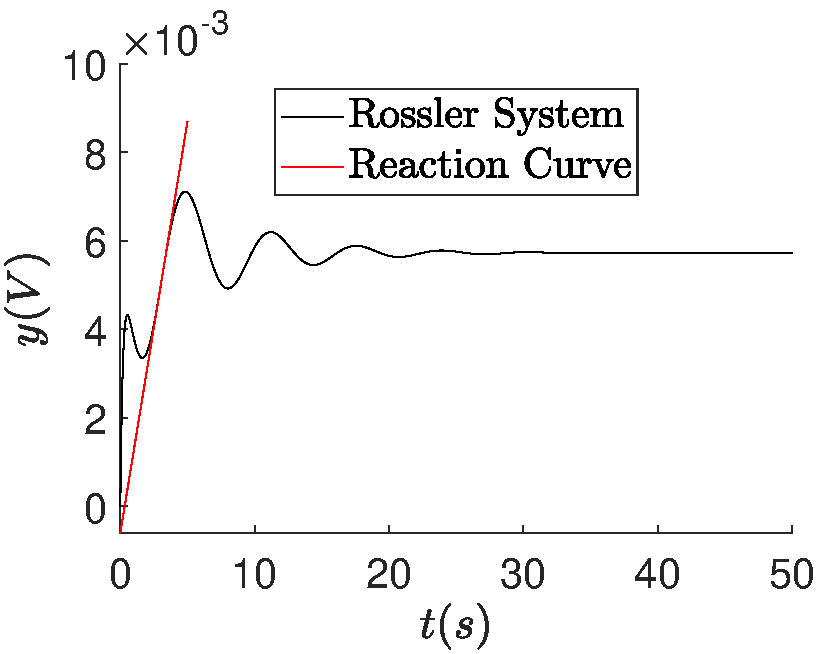
\includegraphics[scale=0.5]{files/reaction_curveRossler.pdf}
    \caption{Reaction curve.}
    \label{fig:reaction_curveRossler}
\end{figure}

Calculating the slope of this line and the delay: $R=0.0019$ and $L=0.8239$. This values yield the following PID parameters:
\begin{equation*}
    \begin{split}
        K_p&=782.8568\\
        T_i&=1.6478\\
        T_d&=0.4119
    \end{split}
\end{equation*}
Applying the formulas for the discrete PID, yields
\begin{equation*}
    \begin{split}
        q_0=&1342.9\\
        q_1=&-1190.3\\
        q_2=&322.4894
    \end{split}
\end{equation*}
Therefore, the transfer function of the discrete PID controller is
\begin{equation}
    \dfrac{U(z)}{E(z)}=\dfrac{1342.9z^2-1190.3z+322.4894}{z(z-1)}
\end{equation}

Now, a simulation applying this controller was performed using as reference $r(t)=1V$, for both the linear and nonlinear systems. In Fig. \ref{fig:zeigler_linear}, the control action and the output of the linear system is presented; note that this PID controller makes the linear system unstable, which is not desired.

    \begin{figure}
        \centering
        \begin{subfigure}[b]{0.475\textwidth}
            \centering
            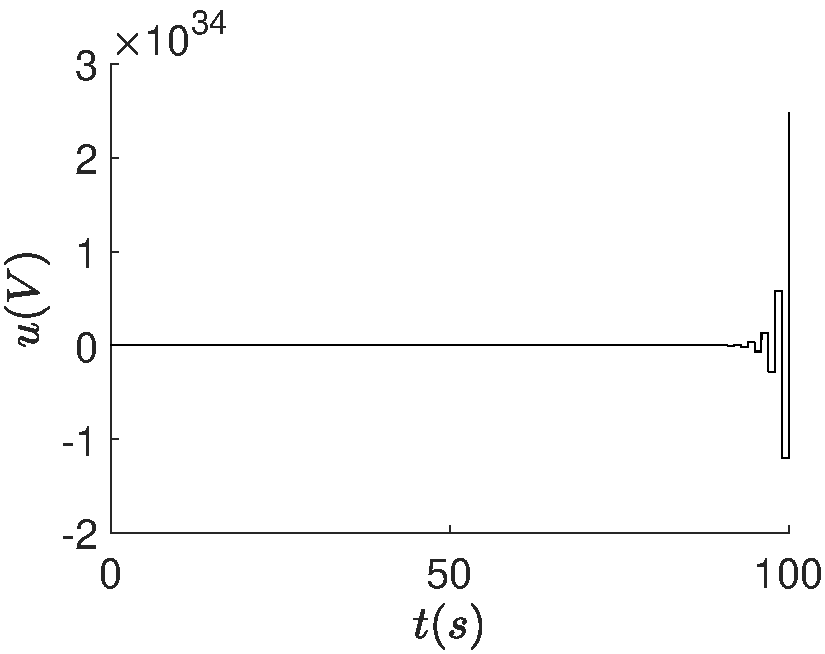
\includegraphics[scale=0.425]{files/heuristic/zeigler/plot_control_zeigler_linear.pdf}
            \caption{Control action.}
        \end{subfigure}
        \vskip0.1cm
        \begin{subfigure}[b]{0.475\textwidth}   
            \centering 
            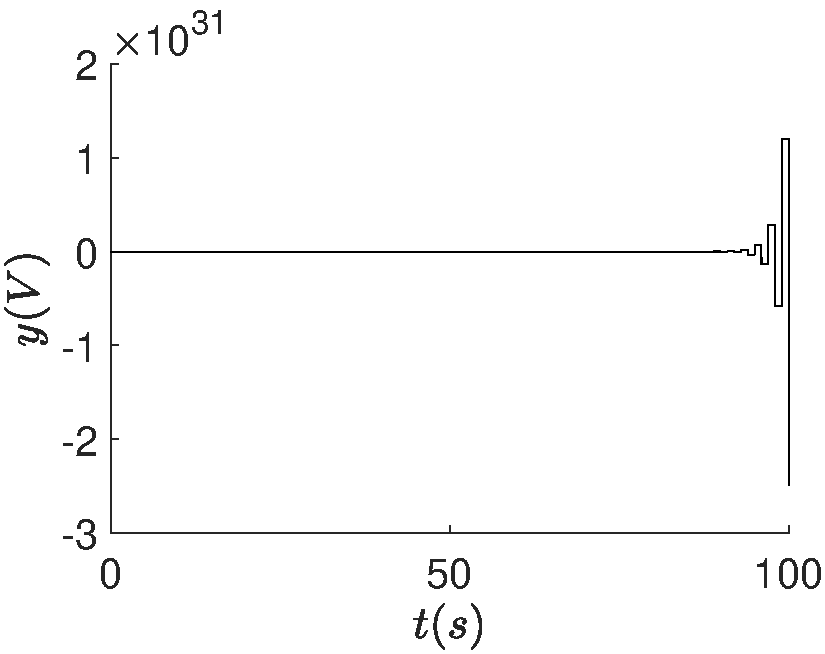
\includegraphics[scale=0.425]{files/heuristic/zeigler/plot_y_zeigler_linear.pdf}
            \caption{Output.}
        \end{subfigure}
        \caption{Linear system simulation with discrete Zeigler-Nichols controller.}
        \label{fig:zeigler_linear}
	\end{figure}
	
	On the other hand, the control action and the output of the nonlinear system is shown in Fig. \ref{fig:zeigler}. It is important to highlight that a saturation was selected for the input, i.e. a minimum and maximum value for the control action was added. This saturation was selected from $0V$ to a maximum of $1500V$, since it is a reasonable interval from a power source as input; note that the control action shown in Fig. \ref{fig:zeigler} a. was extracted before the saturation.
	
    \begin{figure}
        \centering
        \begin{subfigure}[b]{0.475\textwidth}
            \centering
            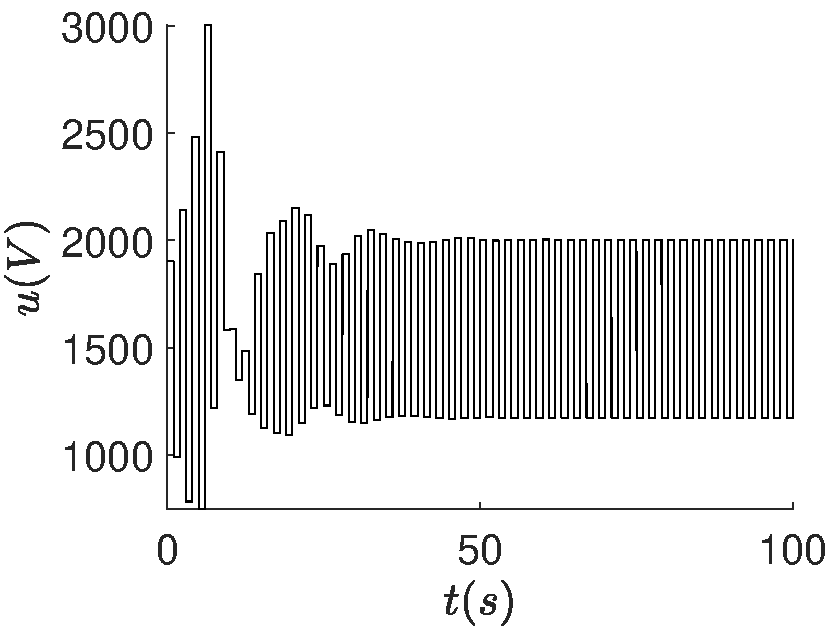
\includegraphics[scale=0.425]{files/heuristic/zeigler/plot_control_zeigler.pdf}
            \caption{Control action.}
        \end{subfigure}
        \vskip0.1cm
        \begin{subfigure}[b]{0.475\textwidth}   
            \centering 
            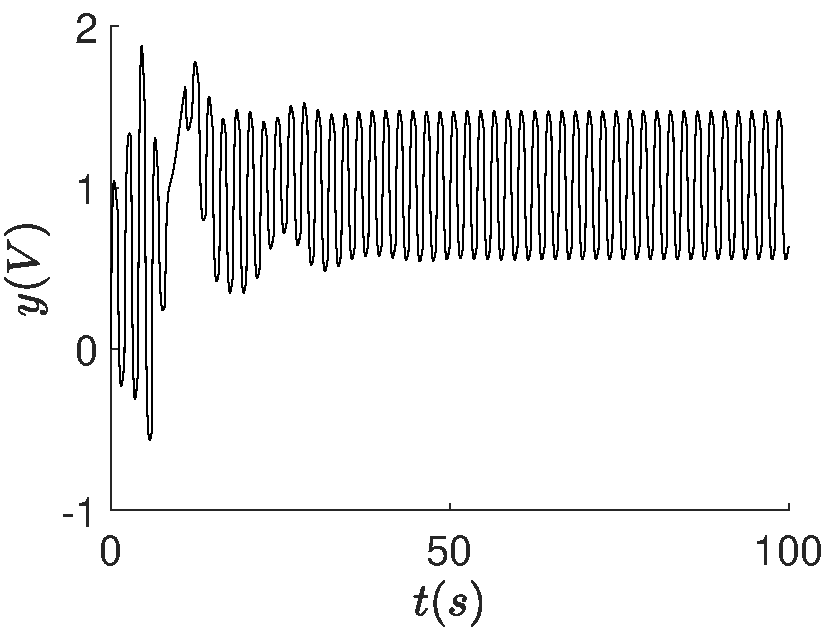
\includegraphics[scale=0.425]{files/heuristic/zeigler/plot_y_zeigler.pdf}
            \caption{Output.}
        \end{subfigure}
        \caption{Rössler system simulation with discrete Zeigler-Nichols controller.}
        \label{fig:zeigler}
	\end{figure}
	
	Moreover, the tuning was performed with the reaction curve but applying the Chien-Hrones-Reswick rules for $0\%$ of maximum overshoot. The discrete PID controller is
	\begin{equation*}
	    \dfrac{U(z)}{E(z)}=\dfrac{990.9356z^2-891.9540z+214.4554}{z(z-1)}
	\end{equation*}
	And the same simulation was performed with $r(t)=1V$. The plots presented in Fig. \ref{fig:chr_linear} show the control action for the linear system applying the Chien-Hrones-Reswick controller. Note that, just as Zeigler-Nichols controller, it makes the linear system unstable.
	
	\begin{figure}
        \centering
        \begin{subfigure}[b]{0.475\textwidth}
            \centering
            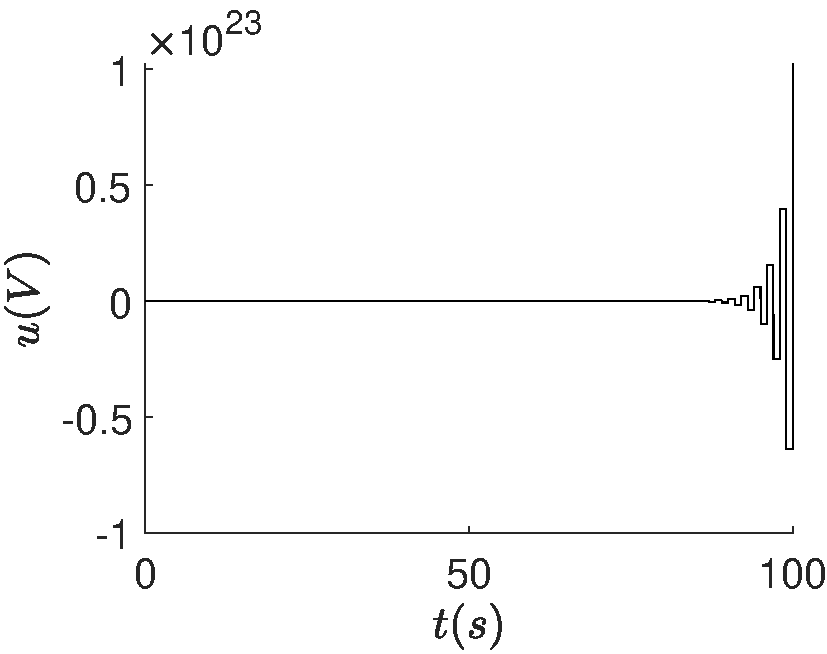
\includegraphics[scale=0.425]{files/heuristic/CHR/plot_control_CHR_linear.pdf}
            \caption{Control action.}
        \end{subfigure}
        \vskip0.1cm
        \begin{subfigure}[b]{0.475\textwidth}   
            \centering 
            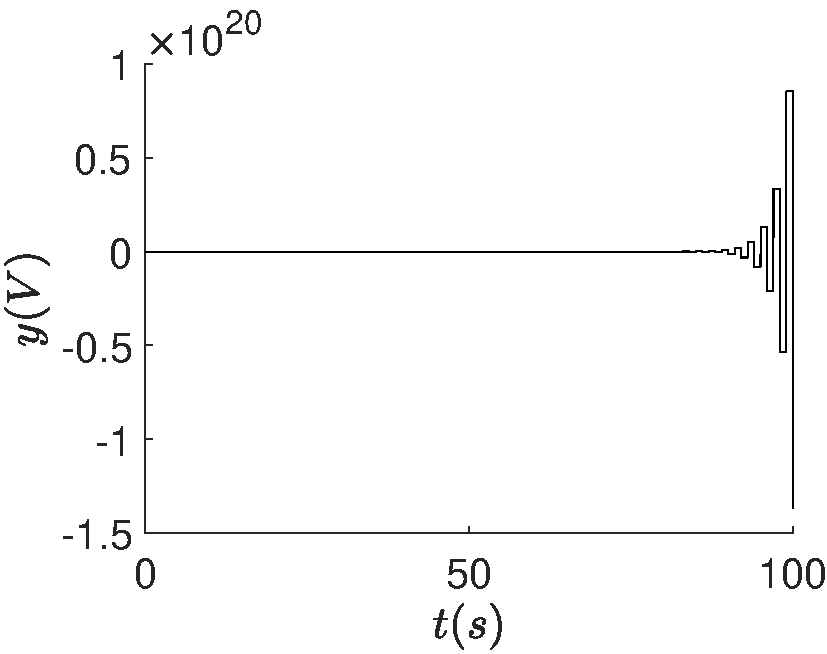
\includegraphics[scale=0.425]{files/heuristic/CHR/plot_y_CHR_linear.pdf}
            \caption{Output.}
        \end{subfigure}
        \caption{Linear system simulation with discrete Chien-Hrones-Reswick controller.}
        \label{fig:chr_linear}
	\end{figure}
    
    Finally, the control action and system output of the Rössler nonlinear equations in study are presented in Fig. \ref{fig:chr}. Again, there is saturation in the control action 
    
    \begin{figure}
        \centering
        \begin{subfigure}[b]{0.475\textwidth}
            \centering
            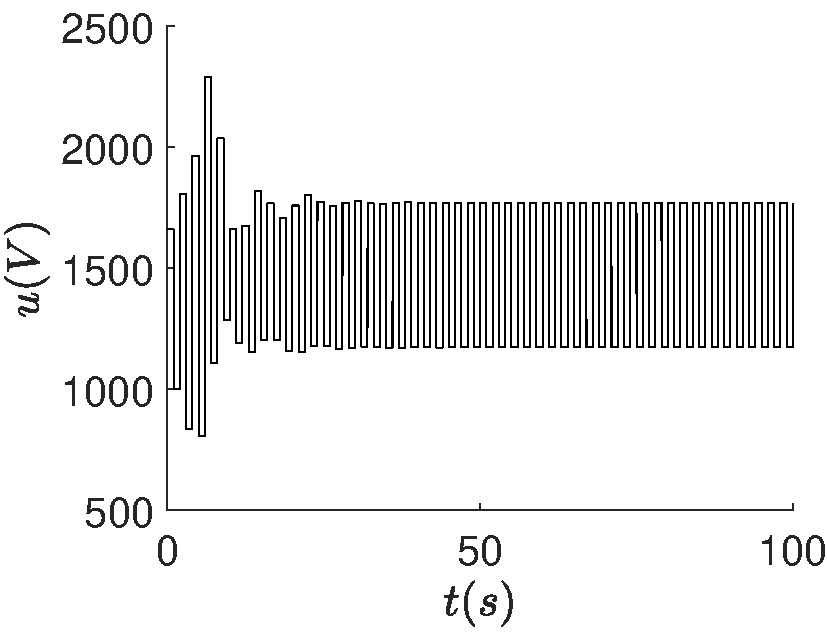
\includegraphics[scale=0.425]{files/heuristic/CHR/plot_control_CHR.pdf}
            \caption{Control action.}
        \end{subfigure}
        \vskip0.1cm
        \begin{subfigure}[b]{0.475\textwidth}   
            \centering 
            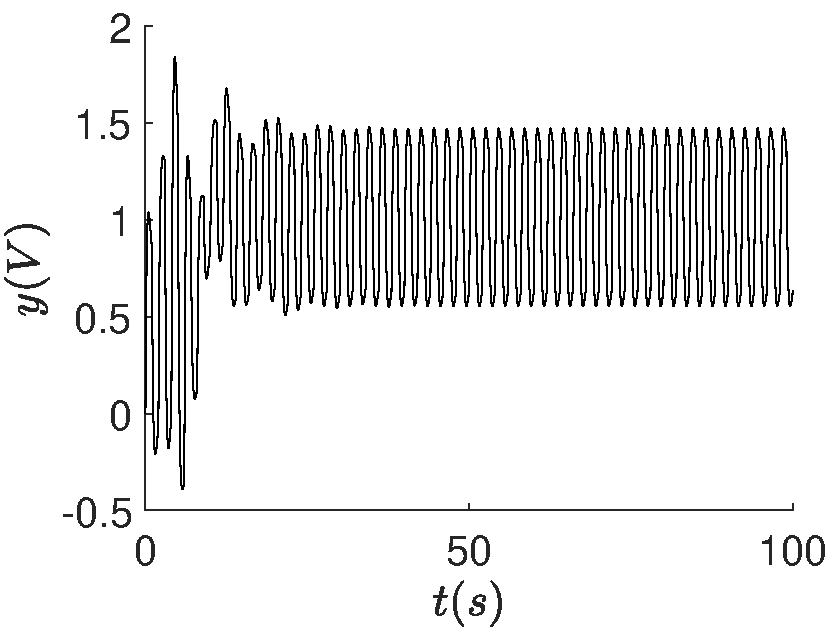
\includegraphics[scale=0.425]{files/heuristic/CHR/plot_y_CHR.pdf}
            \caption{Output.}
        \end{subfigure}
        \caption{Rössler system simulation with discrete Chien-Hrones-Reswick controller.}
        \label{fig:chr}
	\end{figure}


    \subsubsection{Tuning by Sensitivity Curve}
    The second method presented in \ref{sec:tuning} is through the gain margin $M_G$ and its frequency $\omega_{cf}$. In previous work \cite{JS_PL2}, the respective gain margin and frequency was obtained: 
    $M_G=52.7993dB$ and $\omega_{cf}=3.1416rad/s$, which yield $K_u=436.48$ and $T_u=2s$. Therefore, the discrete PID controller with the sensitivity method is
    \begin{equation*}
	    \dfrac{U(z)}{E(z)}=\dfrac{458.3046z^2-261.8883z+65.4721}{z(z-1)}
	\end{equation*}
    In order to make a comparison with the previously obtained PID controllers, the same simulation will be performed with $r(t)=1$. In Fig. \ref{fig:sens}, the control action and output for the nonlinear Rössler system is presented. Note that, unlike the previous PID controllers, this one does not unstabilize the system and can eliminate eliminate steady-state error for this particular reference.
    
    \begin{figure}
        \centering
        \begin{subfigure}[b]{0.475\textwidth}
            \centering
            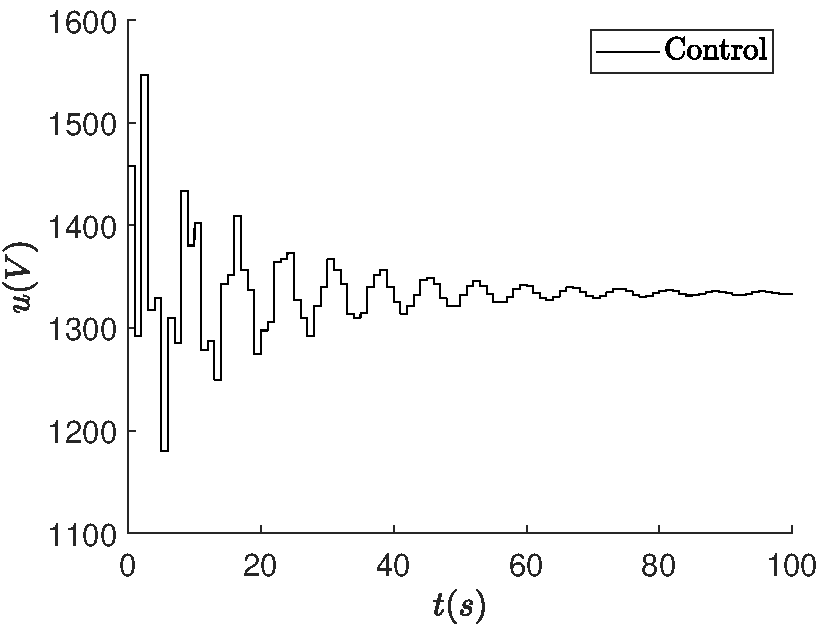
\includegraphics[scale=0.425]{files/heuristic/Sensitivity/control_sens_u_1.pdf}
            \caption{Control action.}
        \end{subfigure}
        \vskip0.1cm
        \begin{subfigure}[b]{0.475\textwidth}   
            \centering 
            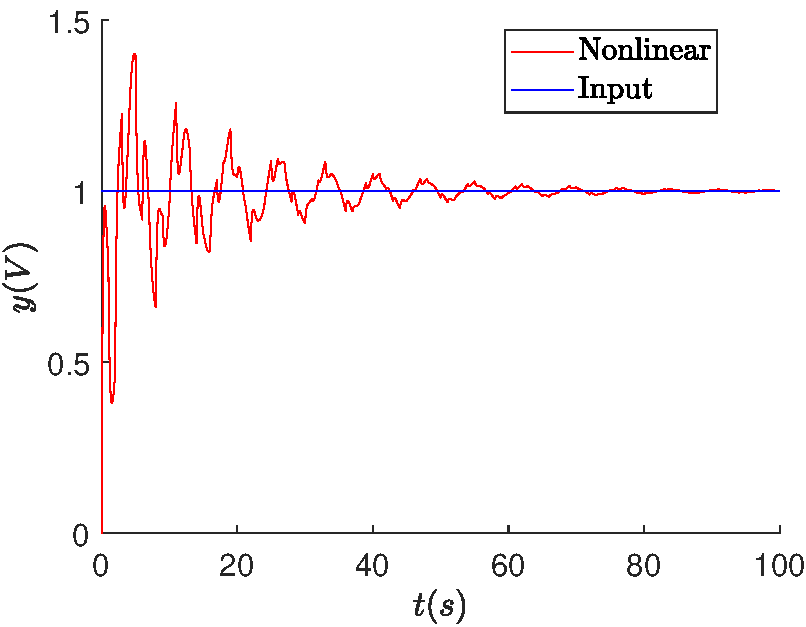
\includegraphics[scale=0.425]{files/heuristic/Sensitivity/sens_u_1.pdf}
            \caption{Output.}
        \end{subfigure}
        \caption{Rössler system simulation with discrete sensitivity controller.}
        \label{fig:sens}
	\end{figure}
	
    It is important to highlight that the linear system is not presented since it works perfectly with this controller. Note that the system shows stabilization in $1V$. Now that a functional controller was found, we proceed to make an analysis on this controller.
    
    In order to start the analysis, the following plots (Fig. \ref{fig:sens_lin_nonlin}) show the steady-state values for the output and the control signal for different inputs; this figure was constructed following the same ideas behind a linearity curve (see \cite{JS_PL2}). Note that the plots show that the nonlinear system diverges from the linear controlled system, due to the saturation defined in the system.
    
    \begin{figure}
        \centering
        \begin{subfigure}[b]{0.475\textwidth}
            \centering
            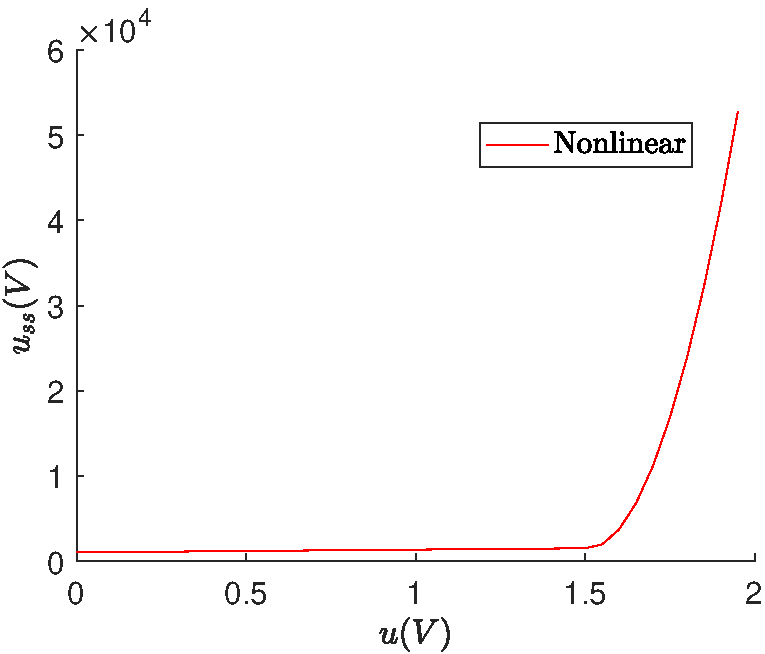
\includegraphics[scale=0.425]{files/heuristic/Sensitivity/control_sens_lin_vs_nonlin.pdf}
            \caption{Control action.}
        \end{subfigure}
        \vskip0.1cm
        \begin{subfigure}[b]{0.475\textwidth}
            \centering 
            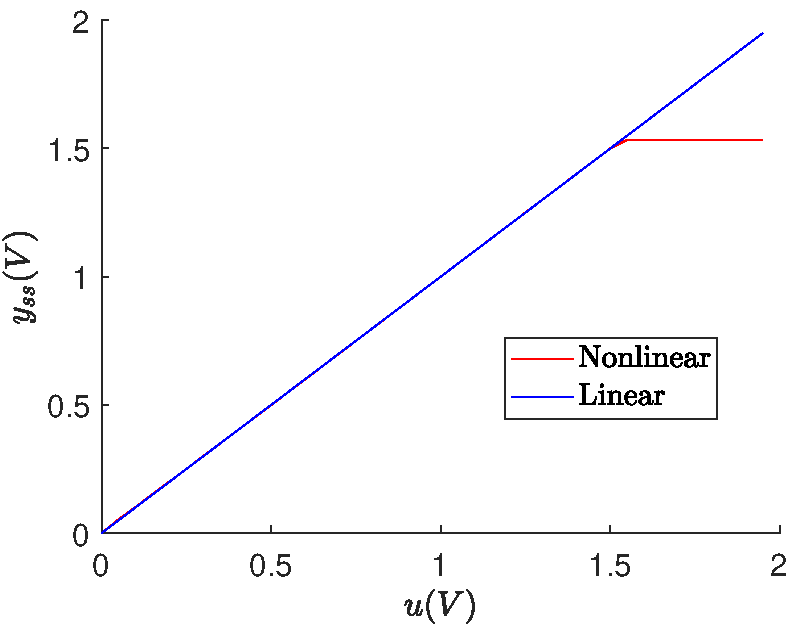
\includegraphics[scale=0.425]{files/heuristic/Sensitivity/sens_lin_vs_nonlin.pdf}
            \caption{Output.}
        \end{subfigure}
        \caption{Sensitivity linear vs. nonlinear system.}
        \label{fig:sens_lin_nonlin}
	\end{figure}
	
    
    Now, it was desired test the controller with time-dependent references. The first simulation was for a reference $r(t)=0.01t$ with $t\in[0,100]$. The result of this simulation for both control and output is presented in Fig. \ref{fig:sens_ref_0_01t}; note that the control system makes a good attempt to stabilize the system exactly at the reference, making the error almost constant. Note that the control action remains inside the saturation interval, meaning that the control does not exceed the predefined limit.
    
    \begin{figure}
        \centering
        \begin{subfigure}[b]{0.475\textwidth}
            \centering
            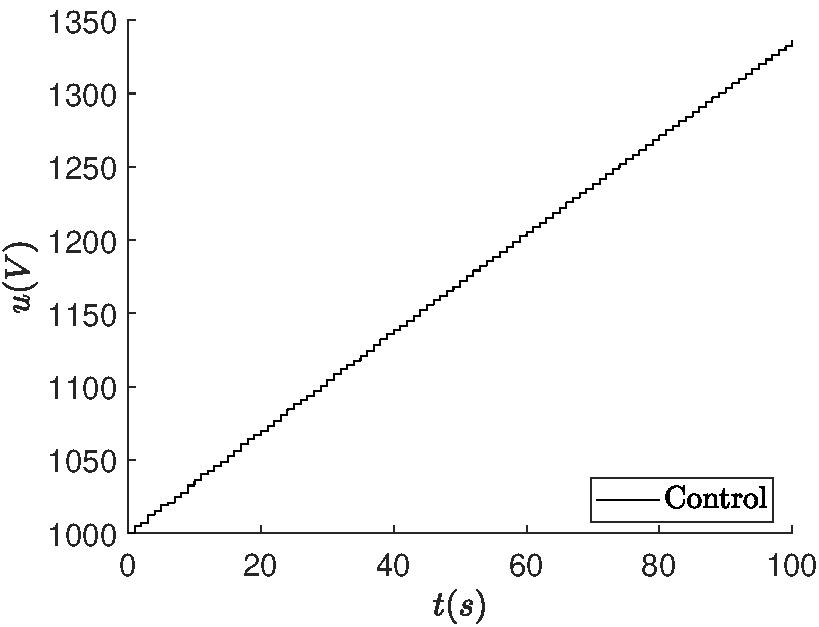
\includegraphics[scale=0.425]{files/heuristic/Sensitivity/control_sens_ramp_ref_0_01.pdf}
            \caption{Control action.}
        \end{subfigure}
        \vskip0.1cm
        \begin{subfigure}[b]{0.475\textwidth}   
            \centering
            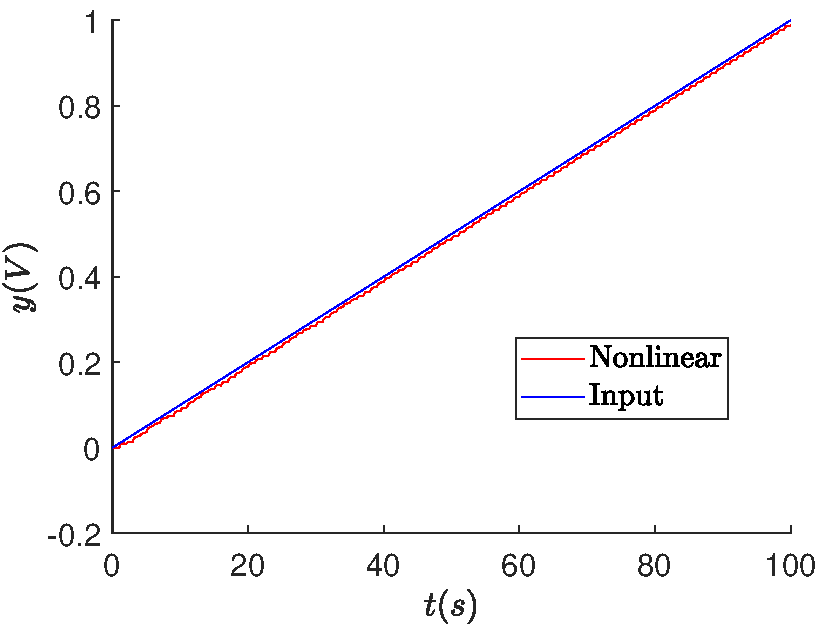
\includegraphics[scale=0.425]{files/heuristic/Sensitivity/sens_ramp_ref_0_01.pdf}
            \caption{Output.}
        \end{subfigure}
        \caption{Rössler system simulation with discrete sensitivity controller for $r(t)=0.01t$.}
        \label{fig:sens_ref_0_01t}
	\end{figure}
    
    Another simulation was executed but for a slightly larger slope: $r(t)=0.018$. The results of this simulation are displayed in Fig. \ref{fig:sens_ref_0_018t}. Note that the control action reaches its maximum value near $90s$, therefore there is saturation and the nonlinear system can no longer ``follow'' the reference, as the output shows: around $90s$ both curves diverge.
    
    \begin{figure}
        \centering
        \begin{subfigure}[b]{0.475\textwidth}
            \centering
            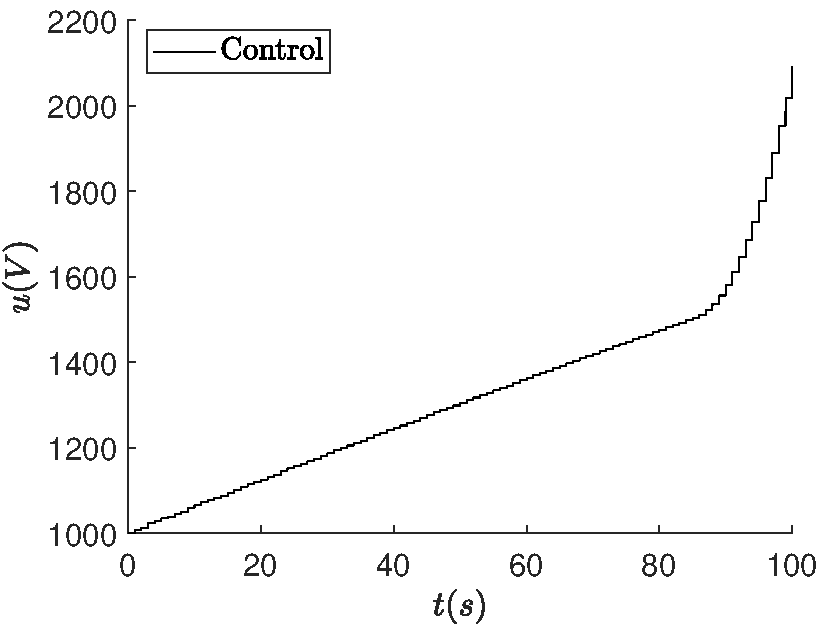
\includegraphics[scale=0.425]{files/heuristic/Sensitivity/control_sens_ramp_ref_0_018.pdf}
            \caption{Control action.}
        \end{subfigure}
        \vskip0.1cm
        \begin{subfigure}[b]{0.475\textwidth}   
            \centering 
            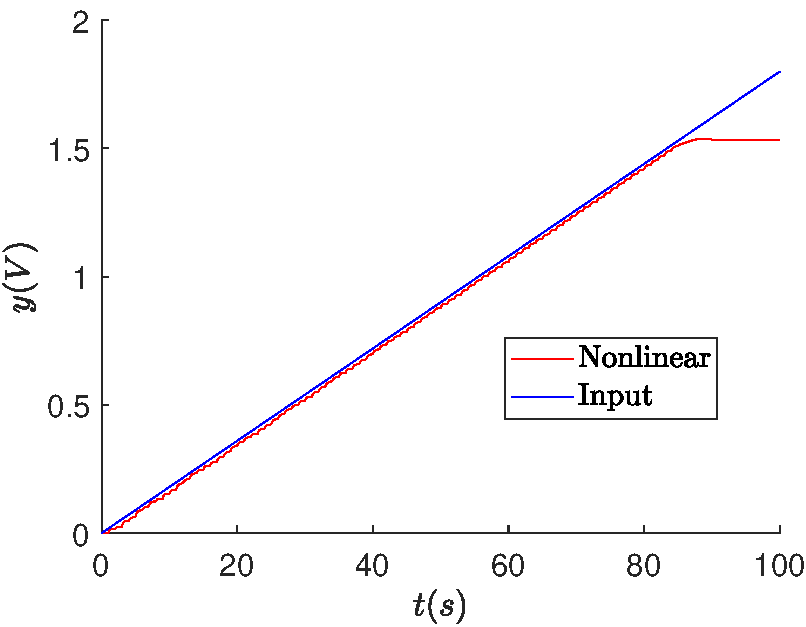
\includegraphics[scale=0.425]{files/heuristic/Sensitivity/sens_ramp_ref_0_018.pdf}
            \caption{Output.}
        \end{subfigure}
        \caption{Rössler system simulation with discrete sensitivity controller for $r(t)=0.018t$.}
        \label{fig:sens_ref_0_018t}
	\end{figure}
    
    As it will be discussed later on the Analysis section \ref{sec:resultAn}, this discrete PID controller has an upper bound. In order to find a lower bound, negative slope references will be analyzed. For a reference of $r(t)=-0.01$, Fig. \ref{fig:sens_ref_-0_01t} shows the control and output; just as its positive counterpart, the nonlinear ``follows'' the negative reference with almost a constant error.
    
    \begin{figure}
        \centering
        \begin{subfigure}[b]{0.475\textwidth}
            \centering
            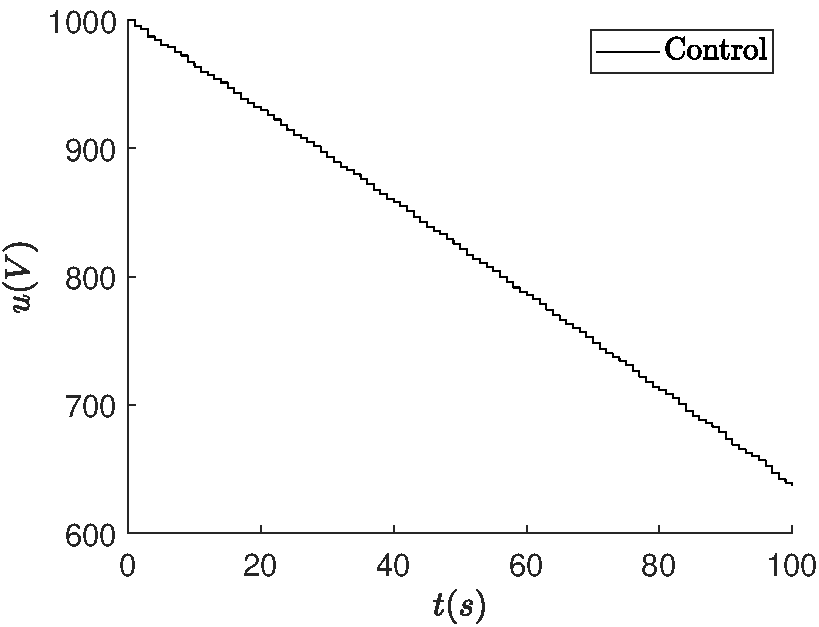
\includegraphics[scale=0.425]{files/heuristic/Sensitivity/control_sens_ramp_ref_-0_01.pdf}
            \caption{Control action.}
        \end{subfigure}
        \vskip0.1cm
        \begin{subfigure}[b]{0.475\textwidth}   
            \centering 
            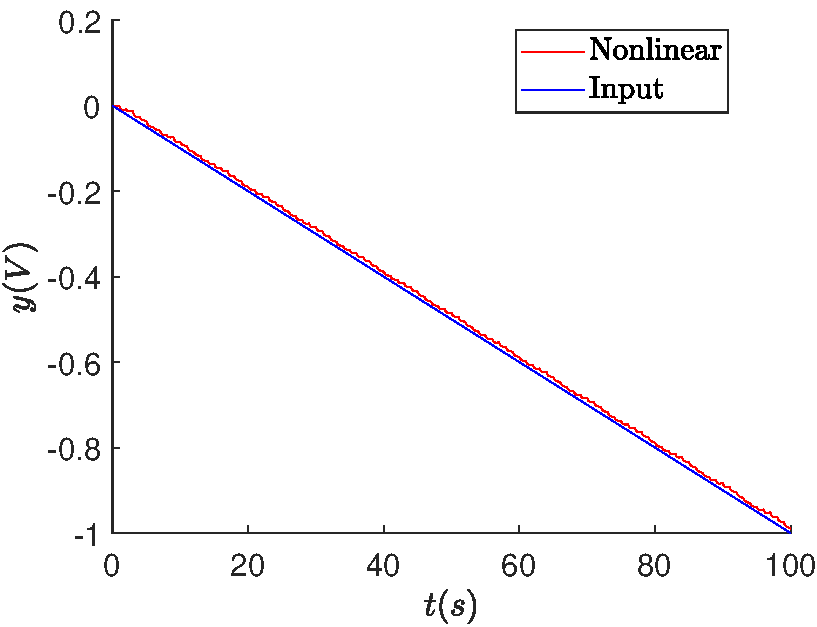
\includegraphics[scale=0.425]{files/heuristic/Sensitivity/sens_ramp_ref_-0_01.pdf}
            \caption{Output.}
        \end{subfigure}
        \caption{Rössler system simulation with discrete sensitivity controller for $r(t)=-0.01t$.}
        \label{fig:sens_ref_-0_01t}
	\end{figure}
	
	For a slightly more negative slope ($r(t)=-0.03t$), the plots presented in Fig. \ref{fig:sens_ref_-0_03t} show that the control action needed is negative, which is a contradiction to the minimum control action set, making the nonlinear system diverge from the reference.
	
	\begin{figure}
        \centering
        \begin{subfigure}[b]{0.475\textwidth}
            \centering
            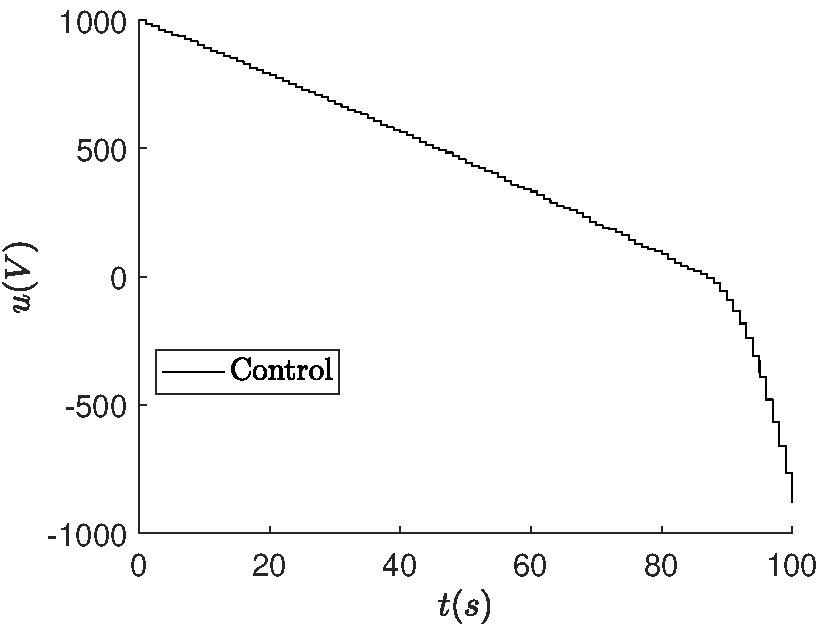
\includegraphics[scale=0.425]{files/heuristic/Sensitivity/control_sens_ramp_ref_-0_03.pdf}
            \caption{Control action.}
        \end{subfigure}
        \vskip0.1cm
        \begin{subfigure}[b]{0.475\textwidth}   
            \centering
            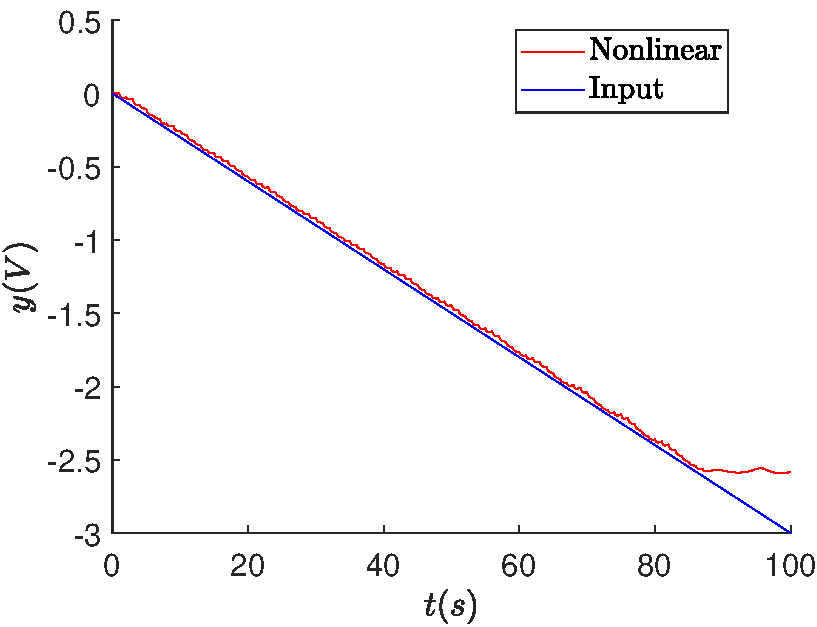
\includegraphics[scale=0.425]{files/heuristic/Sensitivity/sens_ramp_ref_-0_03.pdf}
            \caption{Output.}
        \end{subfigure}
        \caption{Rössler system simulation with discrete sensitivity controller for $r(t)=-0.03t$.}
        \label{fig:sens_ref_-0_03t}
	\end{figure}
	
	For a better visualization of the effect of this lower saturation, one last simulation was performed with the discrete sensitivity PID controller with $r(t)=-0.05t$; Fig. \ref{fig:sens_ref_-0_05t} shows the results. Note that the control action is negative from around $50s$, at that exact time the nonlinear Rössler system diverges completely from the reference and starts to behave chaotically.
    
    \begin{figure}
        \centering
        \begin{subfigure}[b]{0.475\textwidth}
            \centering
            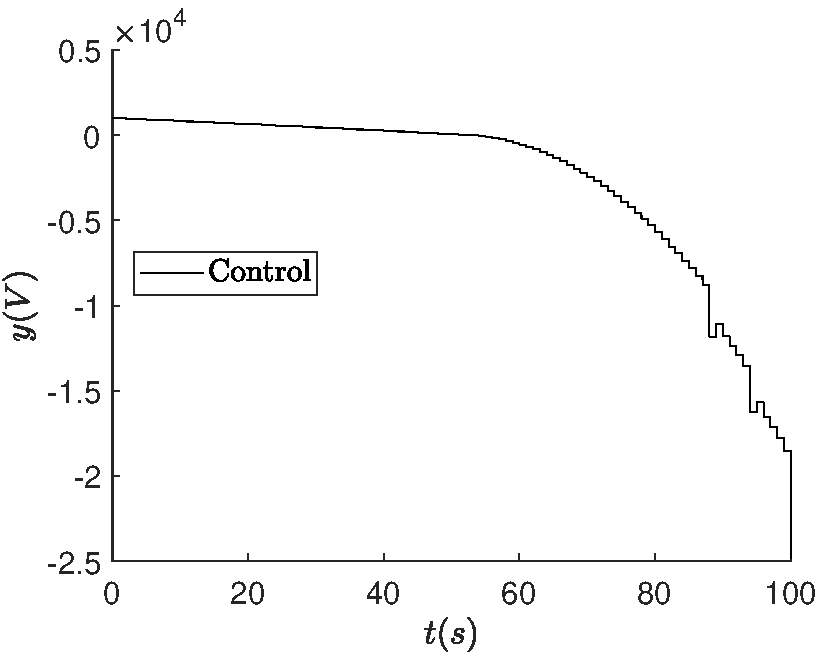
\includegraphics[scale=0.425]{files/heuristic/Sensitivity/control_sens_ramp_ref_-_0_05.pdf}
            \caption{Control action.}
        \end{subfigure}
        \vskip0.1cm
        \begin{subfigure}[b]{0.475\textwidth}   
            \centering 
            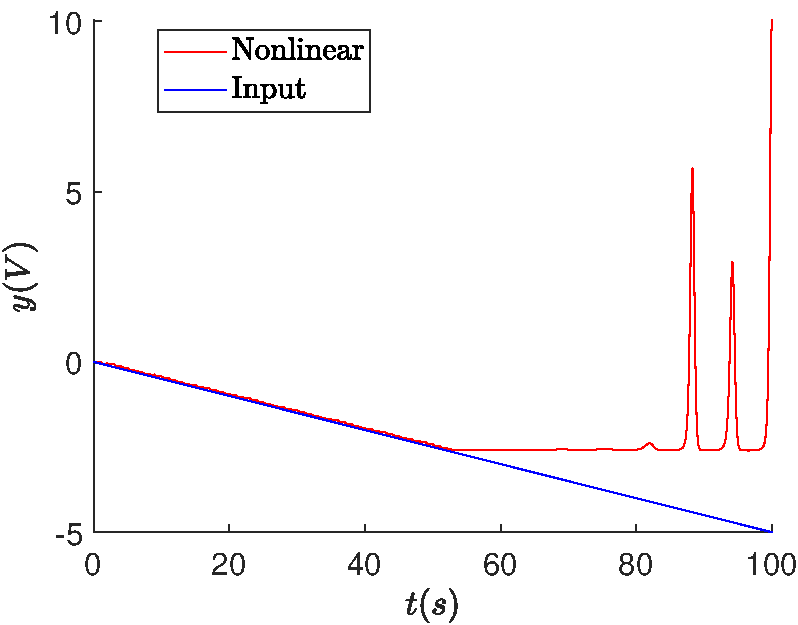
\includegraphics[scale=0.425]{files/heuristic/Sensitivity/sens_ramp_ref_-0_05.pdf}
            \caption{Output.}
        \end{subfigure}
        \caption{Rössler system simulation with discrete sensitivity controller for $r(t)=-0.05t$.}
        \label{fig:sens_ref_-0_05t}
	\end{figure}
    
    Finally, a lower bound for the reference was found by iterative simulation: $r(t)=-0.25$; Fig. \ref{fig:sens_ref_lower} shows the control action and output with the sensitivity discrete PID controller on its critically stable state.
    
    \begin{figure}
        \centering
        \begin{subfigure}[b]{0.475\textwidth}
            \centering
            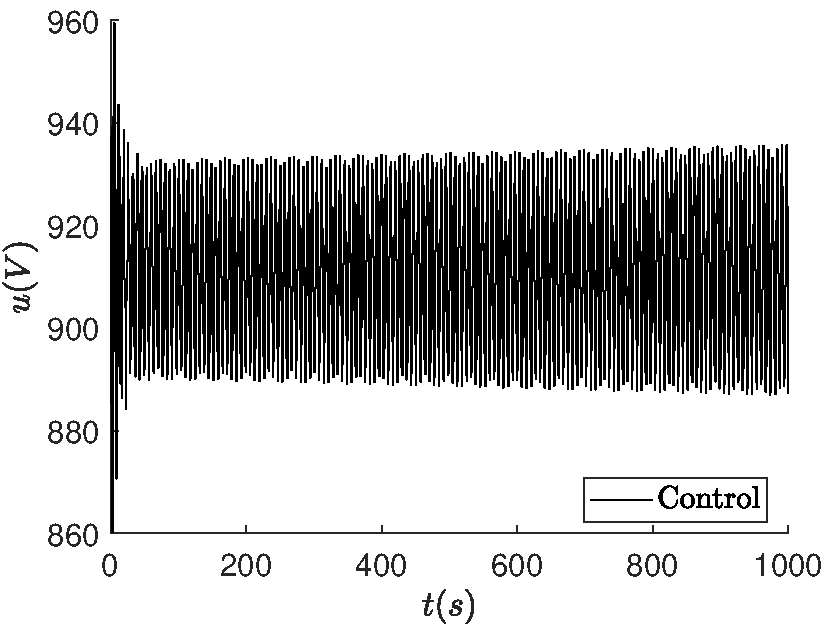
\includegraphics[scale=0.425]{files/heuristic/Sensitivity/control_sens_low_bound_ref.pdf}
            \caption{Control action.}
        \end{subfigure}
        \vskip0.1cm
        \begin{subfigure}[b]{0.475\textwidth}   
            \centering 
            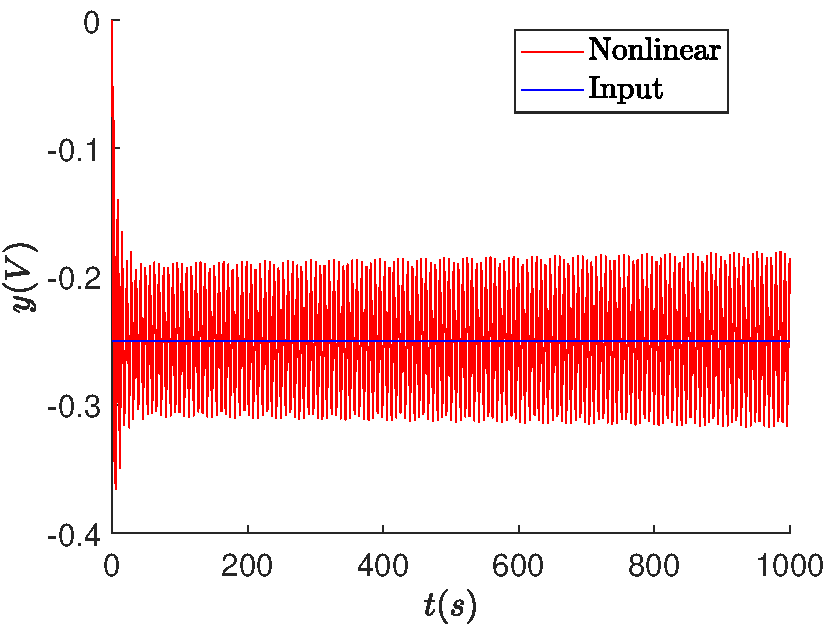
\includegraphics[scale=0.425]{files/heuristic/Sensitivity/sens_u_-0_25.pdf}
            \caption{Output.}
        \end{subfigure}
        \caption{Rössler system simulation with discrete sensitivity controller for $r(t)=-0.25t$.}
        \label{fig:sens_ref_lower}
	\end{figure}
    
    %%%%%%%%%%%%%%%%%%%%%%%
    \subsubsection{Tuning by Analytic Procedure}
    In previous work \cite{JS_PL2}, a second order approximation for the linearized Rössler system was found and has the following transfer function:
    \begin{equation}\label{eq:reduced_order2}
    \tilde{G}(s)=\dfrac{0.001461}{s^2 + 0.5887 s + 0.5102}
    \end{equation}
    and applying a discretization of this transfer function with sample time of $T=1s$, the following discrete system was obtained:
    \begin{equation}
    \tilde{G}(z) = \dfrac{0.000582z+0.0004769}{z^2-1.185z+0.5547}
    \end{equation}
    
    
    The analytic procedure was applied setting all four poles in $0.5$ (closed-loop system), which yields the following discrete PID controller
    \begin{equation}
    \dfrac{U(z)}{E(z)}=\dfrac{212.6018z^2-355.9319z+202.3534}{(z+0.0613)(z-1)}
    \end{equation}
    
    With the obtained discrete PID controller, a simulation was performed for a reference of $r(t)=0.5$ (Fig. \ref{fig:anal_u_0_5}), note that the output is fast and it does not have steady-state error but the response shows high frequency oscillations.
    \begin{figure}
        \centering
        \begin{subfigure}[b]{0.475\textwidth}
            \centering
            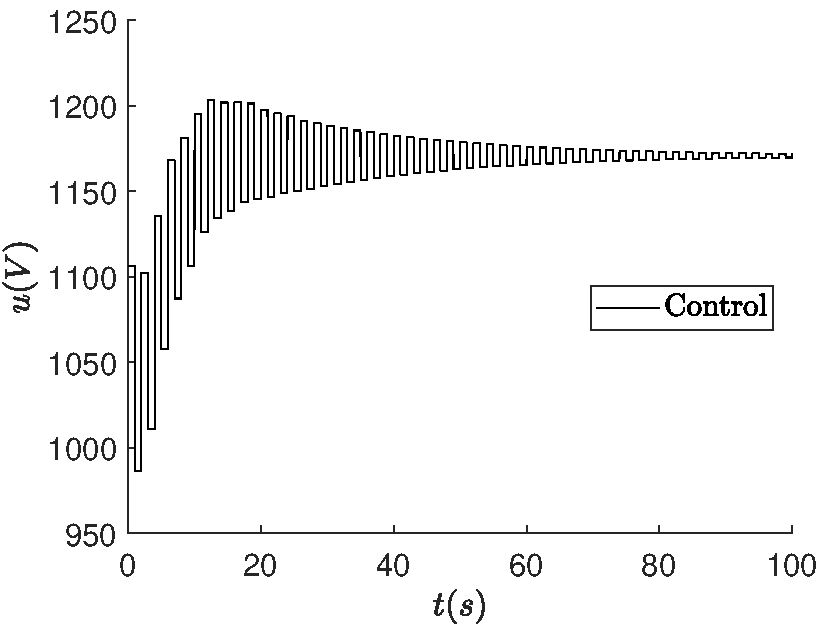
\includegraphics[scale=0.425]{files/heuristic/analytic/control_analytic_u_0_5.pdf}
            \caption{Control action.}
        \end{subfigure}
        \vskip0.1cm
        \begin{subfigure}[b]{0.475\textwidth}   
            \centering 
            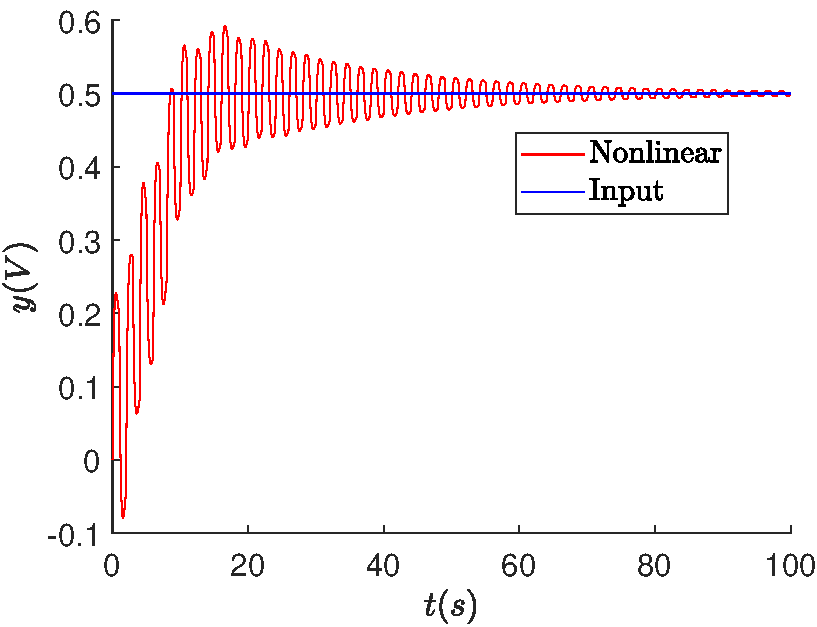
\includegraphics[scale=0.425]{files/heuristic/analytic/analytic_u_0_5.pdf}
            \caption{Output.}
        \end{subfigure}
        \caption{Rössler system simulation with discrete analytic controller for $r(t)=0.5$.}
        \label{fig:anal_u_0_5}
	\end{figure}
	
	Next, a simulation for $r(t)=1.5$ was performed and presented in Fig. \ref{fig:anal_u_1_5}. Notice the high frequency oscillation in transitory state but the smooth stabilization exactly at $1.5$, eliminating the steady-state error.
	\begin{figure}
        \centering
        \begin{subfigure}[b]{0.475\textwidth}
            \centering
            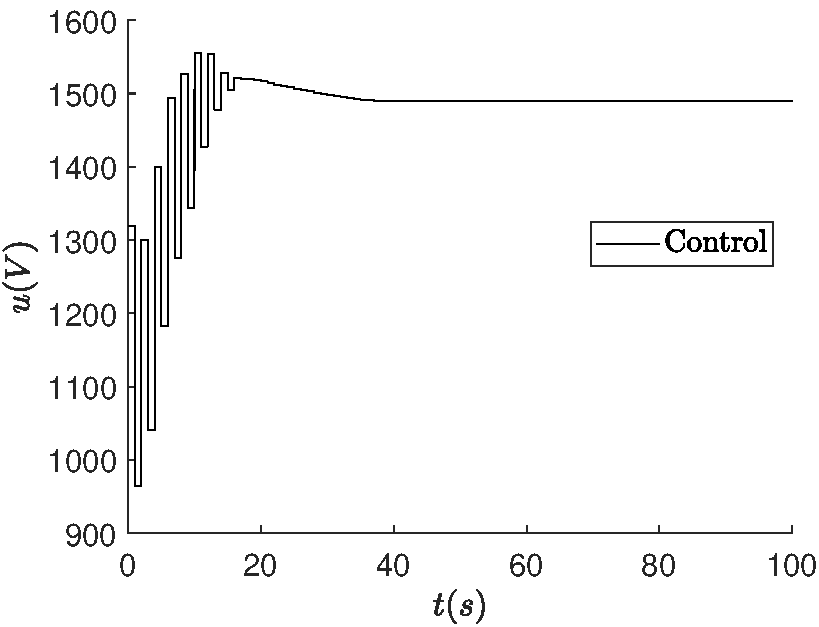
\includegraphics[scale=0.425]{files/heuristic/analytic/control_analytic_u_1_5.pdf}
            \caption{Control action.}
        \end{subfigure}
        \vskip0.1cm
        \begin{subfigure}[b]{0.475\textwidth}   
            \centering 
            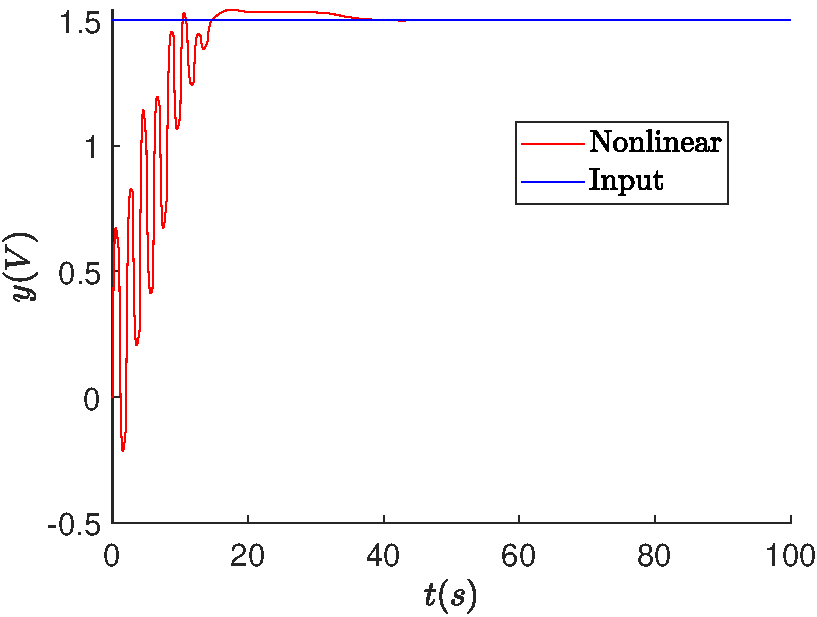
\includegraphics[scale=0.425]{files/heuristic/analytic/analytic_u_1_5.pdf}
            \caption{Output.}
        \end{subfigure}
        \caption{Rössler system simulation with discrete analytic controller for $r(t)=1.5$.}
        \label{fig:anal_u_1_5}
	\end{figure}
	
	Finally, another simulation was executed for a negative reference value of $r(t)=-1.2$. The control action and the system output are shown in Fig. \ref{fig:anal_u_-1_2}. This time response is quite fast and shows high frequency oscillation as well. The system does not present steady-state error.
	\begin{figure}
        \centering
        \begin{subfigure}[b]{0.475\textwidth}
            \centering
            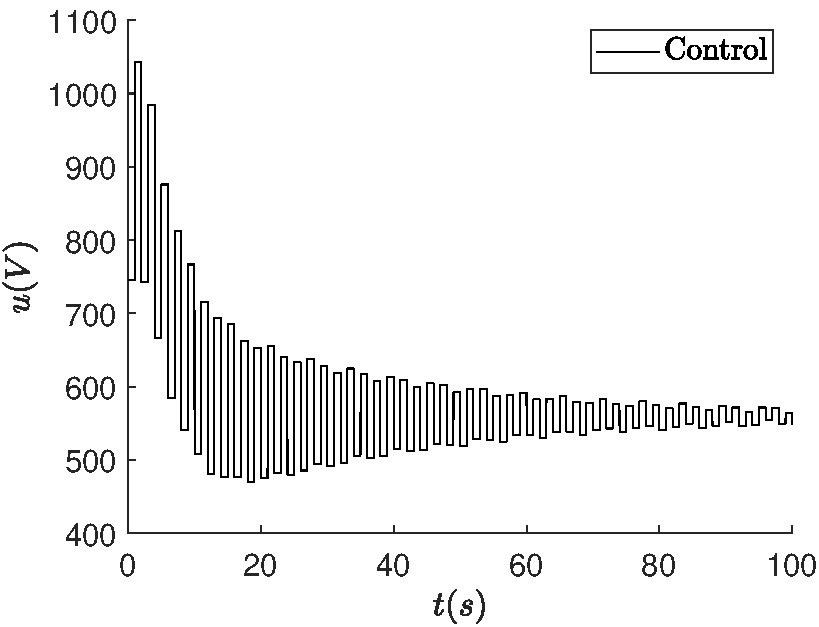
\includegraphics[scale=0.425]{files/heuristic/analytic/control_analytic_u_-1_2.pdf}
            \caption{Control action.}
        \end{subfigure}
        \vskip0.1cm
        \begin{subfigure}[b]{0.475\textwidth}   
            \centering 
            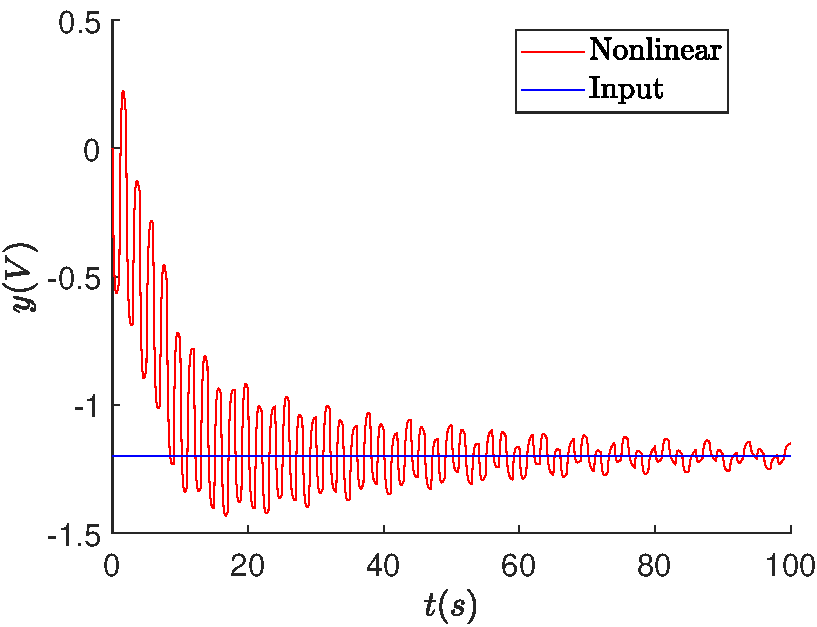
\includegraphics[scale=0.425]{files/heuristic/analytic/analytic_u_-1_2.pdf}
            \caption{Output.}
        \end{subfigure}
        \caption{Rössler system simulation with discrete analytic controller for $r(t)=-1.2$.}
        \label{fig:anal_u_-1_2}
	\end{figure}
	
	Moreover, it was attempted to take the poles to $z=0.4$, which yields the following PID controller
	\begin{equation}
    \dfrac{U(z)}{E(z)}=\dfrac{547.6520z^2-788.6674z+363.4062}{(z+0.2663)(z-1)}
	\end{equation}
    In order to test this controller, a reference of $r(t)=0.5$ was used for the simulation presented in Fig. \ref{fig:anal_u_0_5_poles_0_4}; this simulation shows that the PID controller fails and does not behave properly.
	
	\begin{figure}
        \centering
        \begin{subfigure}[b]{0.475\textwidth}
            \centering
            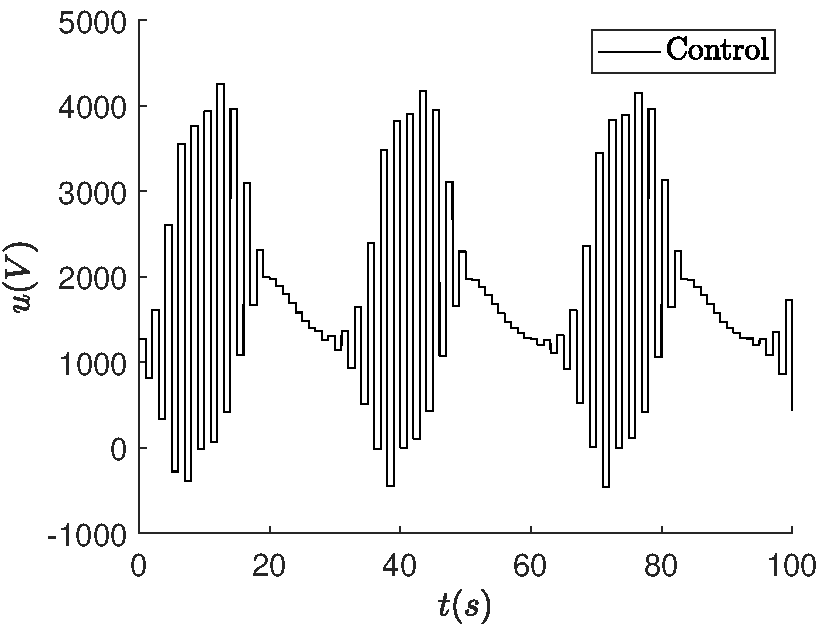
\includegraphics[scale=0.425]{files/heuristic/analytic/control_analytic_u_0_5_poles_0_4.pdf}
            \caption{Control action.}
        \end{subfigure}
        \vskip0.1cm
        \begin{subfigure}[b]{0.475\textwidth}   
            \centering 
            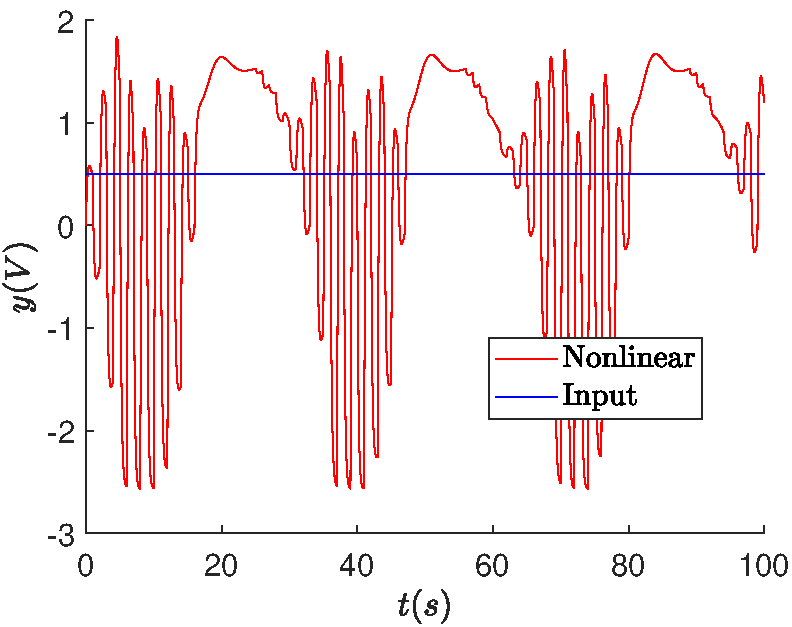
\includegraphics[scale=0.425]{files/heuristic/analytic/analytic_u_0_5_poles_0_4.pdf}
            \caption{Output.}
        \end{subfigure}
        \caption{Rössler system simulation with discrete analytic controller for $r(t)=0.5$ with poles in $0.4$.}
        \label{fig:anal_u_0_5_poles_0_4}
	\end{figure}
	
	
	\subsection{Discrete State Feedback Controller: Pole Assignment}
	It was desired to set the poles exactly at the origin, in $z=0$ (dead-beat controller), with the state feedback control scheme. Applying the method described in \ref{sec:state_feed}, the obtained gain vector is
    \begin{equation}
        K=[-438.5251,\,-103.1074,\,86.1249]
    \end{equation}
	
	
	In order to test the obtained controller, some simulations were performed. Keep in mind that this method is only for $r(t)=0$, therefore the simulations are performed changing the initial conditions for the state $x_3$ (output). The first change is in $0.1V$ and the obtained results are presented in Fig. \ref{fig:feedback_ref0_x30_1}.
	\begin{figure}
        \centering
        \begin{subfigure}[b]{0.475\textwidth}
            \centering
            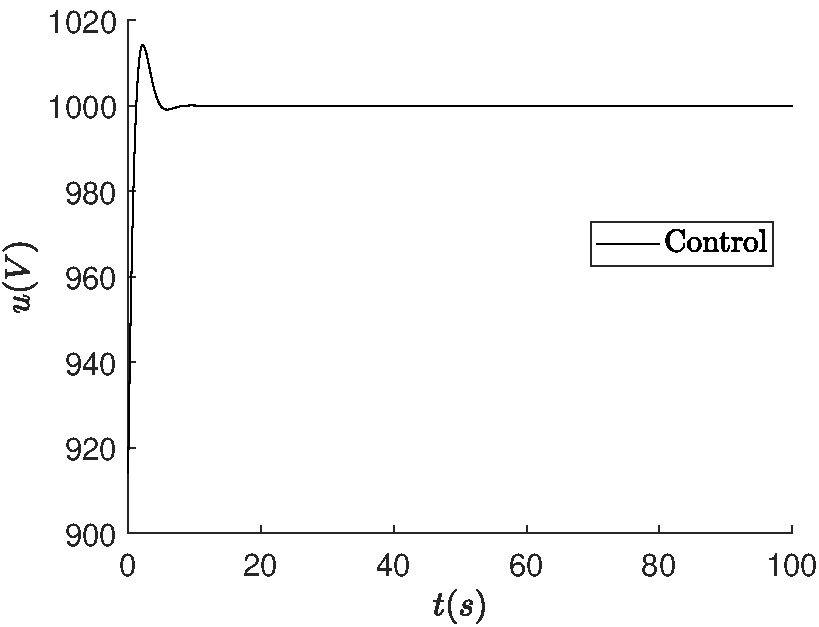
\includegraphics[scale=0.425]{files/feedback/Ref0/control_sfc_x30_1_ref_0.pdf}
            \caption{Control action.}
        \end{subfigure}
        \vskip0.1cm
        \begin{subfigure}[b]{0.475\textwidth}   
            \centering 
            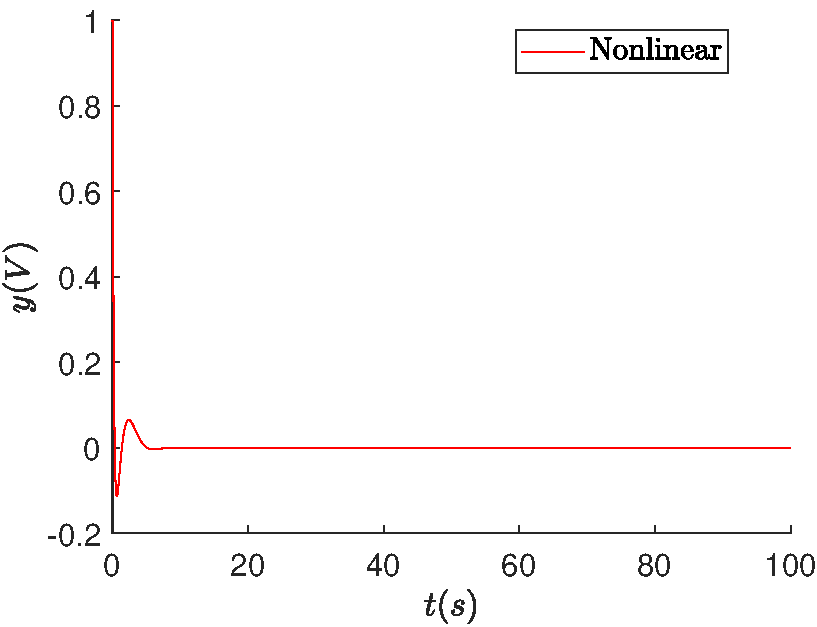
\includegraphics[scale=0.425]{files/feedback/Ref0/sfc_x30_1_ref_0.pdf}
            \caption{Output.}
        \end{subfigure}
        \caption{Rössler system simulation with discrete state feedback controller with $0.1$ in $x_3$.}
        \label{fig:feedback_ref0_x30_1}
	\end{figure}
	
	Next, a simulation changing $50$ in the initial conditions of $x_3$ was carried out; in Fig. \ref{fig:feedback_ref0_x30_5} the control action and the system output can be appreciated. Note that the system can eliminate steady-state error but at the very beginning there is saturation.
	\begin{figure}
        \centering
        \begin{subfigure}[b]{0.475\textwidth}
            \centering
            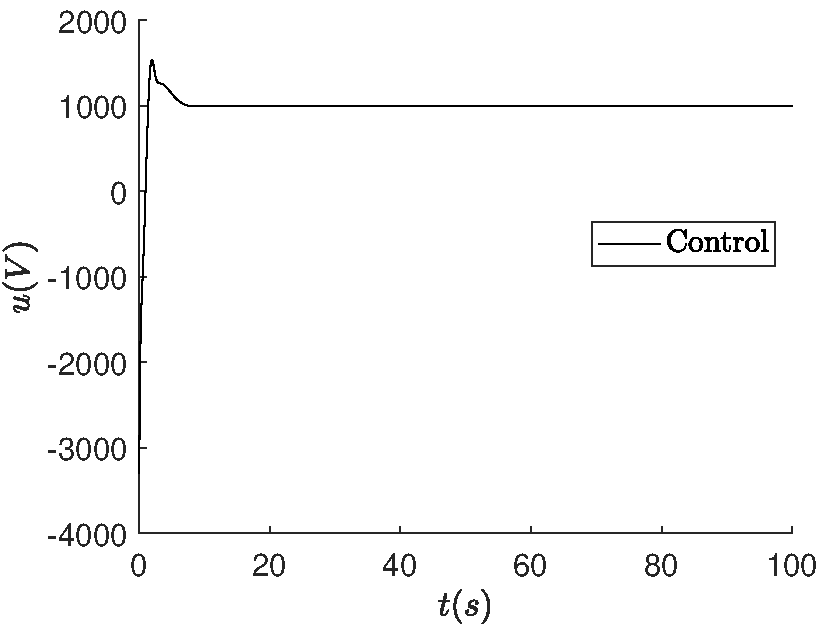
\includegraphics[scale=0.425]{files/feedback/Ref0/control_sfc_x30_50_ref_0.pdf}
            \caption{Control action.}
        \end{subfigure}
        \vskip0.1cm
        \begin{subfigure}[b]{0.475\textwidth}   
            \centering 
            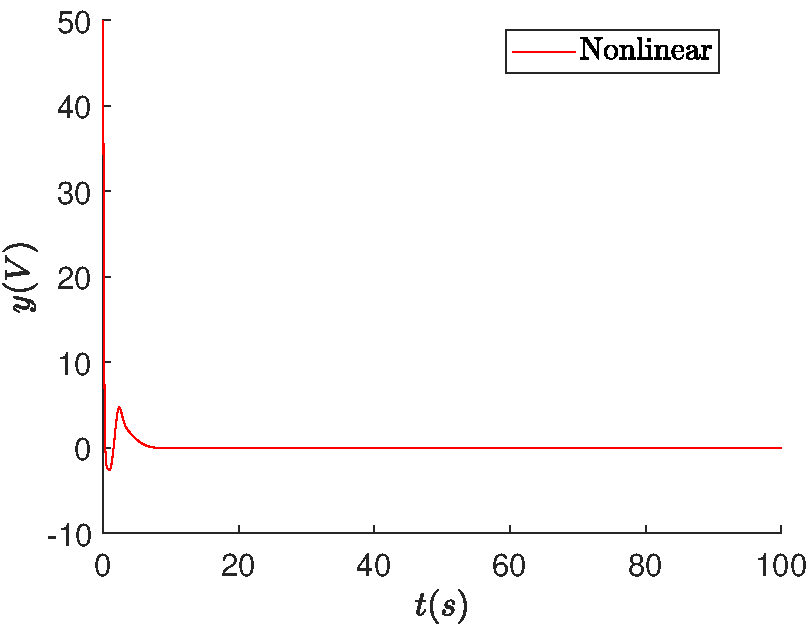
\includegraphics[scale=0.425]{files/feedback/Ref0/sfc_x30_50_ref_0.pdf}
            \caption{Output.}
        \end{subfigure}
        \caption{Rössler system simulation with discrete state feedback controller with $50$ in $x_3$.}
        \label{fig:feedback_ref0_x30_5}
	\end{figure}
	
	Now, testing for a negative change in the initial condition, it was subtracted $2.6$ from the initial conditions of $x_3$. In Fig. \ref{fig:feedback_ref0_x3-0_26} these results are presented for the control and the output. Note that there is no saturation neither steady-state error.
	\begin{figure}
        \centering
        \begin{subfigure}[b]{0.475\textwidth}
            \centering
            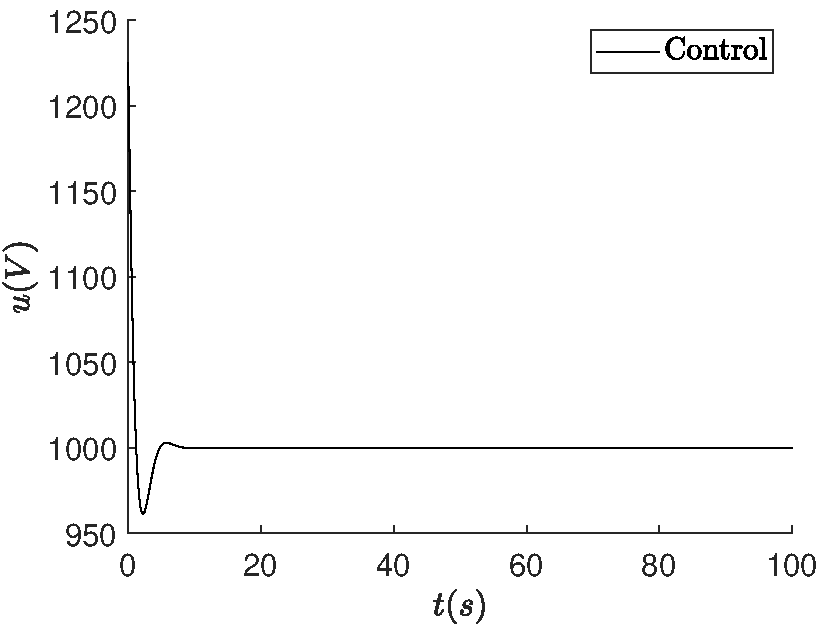
\includegraphics[scale=0.425]{files/feedback/Ref0/control_sfc_x30_-2_6_ref_0.pdf}
            \caption{Control action.}
        \end{subfigure}
        \vskip0.1cm
        \begin{subfigure}[b]{0.475\textwidth}   
            \centering 
            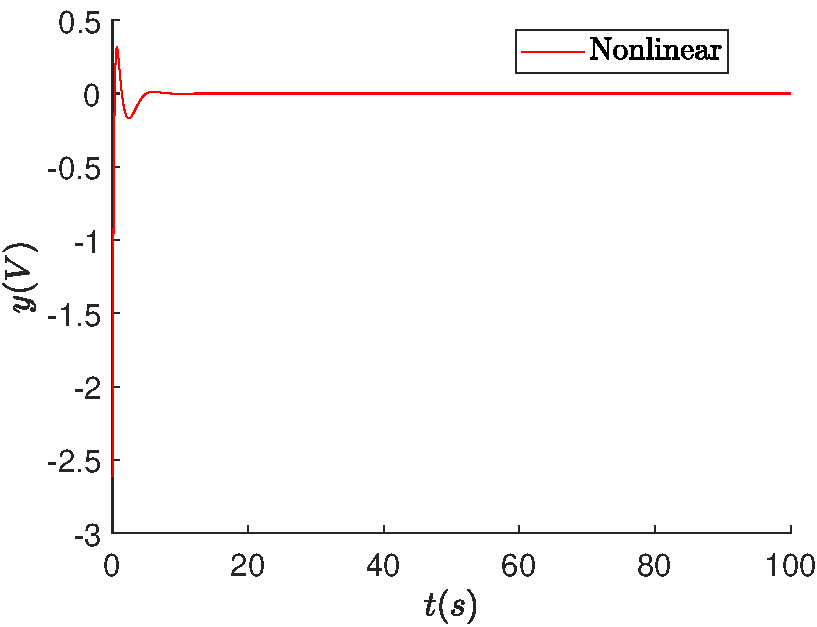
\includegraphics[scale=0.425]{files/feedback/Ref0/sfc_x30_-2_6_ref_0.pdf}
            \caption{Output.}
        \end{subfigure}
        \caption{Rössler system simulation with discrete state feedback controller with $-2.6$ in $x_3$.}
        \label{fig:feedback_ref0_x3-0_26}
	\end{figure}
	
    \subsection{Discrete State Feedback Controller: Pole Assignment without $e_{ss}$}
    In this section, all the desired poles for the system were $z=0.5$ (prior analysis yielded that $z=0$ required way too much energy). Carrying out the procedures depicted in section \ref{sec:state_feed_noess}, the gain vectors are
	\begin{equation}
	\begin{split}
	    K=&[-24.9703,\,156.6863,\,14.2350]\\
	    L=&-28.1628
	\end{split}
	\end{equation}
	
	It has been mentioned that this controller allows for $r(t)\neq0$; therefore, in order to test this controller and to compare with the previously obtained ones, a simulation was conducted using $r(t)=1$. The results for said simulation are shown in Fig. \ref{fig:feedback_u_1}. Note that this controller is achieves stability and can eliminate steady-state error for $r(t)=1$.
	
	\begin{figure}
        \centering
        \begin{subfigure}[b]{0.475\textwidth}
            \centering
            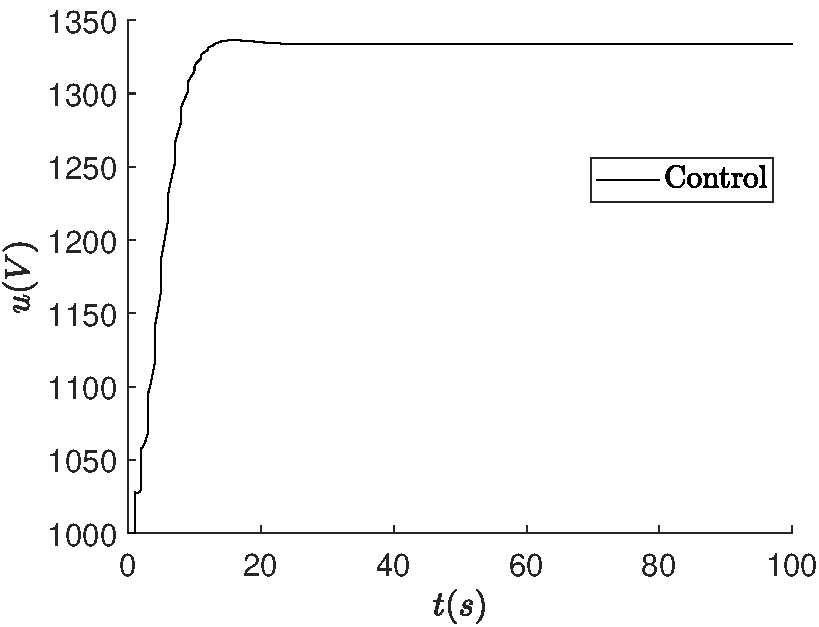
\includegraphics[scale=0.425]{files/feedback/Ref!0/control_sfc_u_1_ref_dif_0.pdf}
            \caption{Control action.}
        \end{subfigure}
        \vskip0.1cm
        \begin{subfigure}[b]{0.475\textwidth}   
            \centering 
            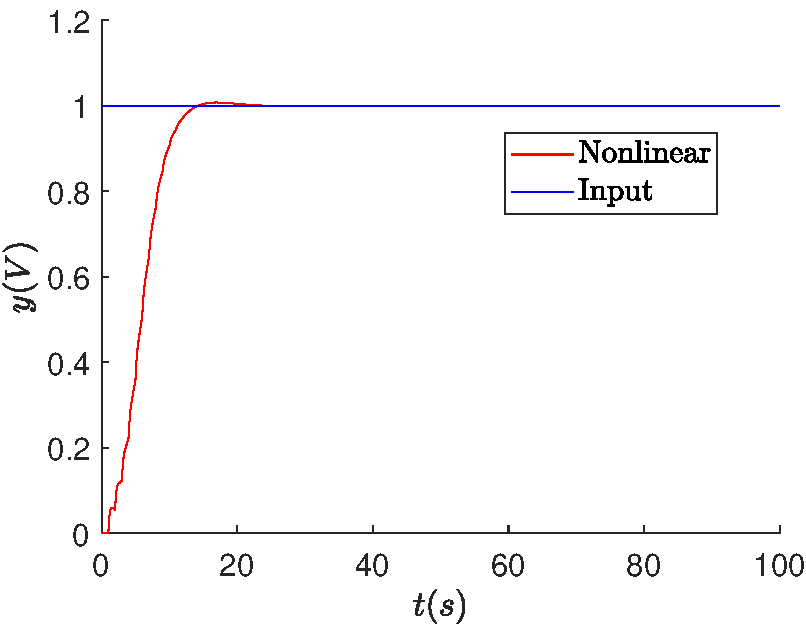
\includegraphics[scale=0.425]{files/feedback/Ref!0/sfc_u_1_ref_dif_0.pdf}
            \caption{Output.}
        \end{subfigure}
        \caption{Rössler system simulation with discrete state feedback controller $r(t)=1$.}
        \label{fig:feedback_u_1}
	\end{figure}
	
	Another simulation was performed using $r(t)=1.5$ (Fig. \ref{fig:feedback_u_1_5}) and the system showed proper behavior with this controller, eliminating steady-state error but with slightly larger overshoot without saturation.
	\begin{figure}
        \centering
        \begin{subfigure}[b]{0.475\textwidth}
            \centering
            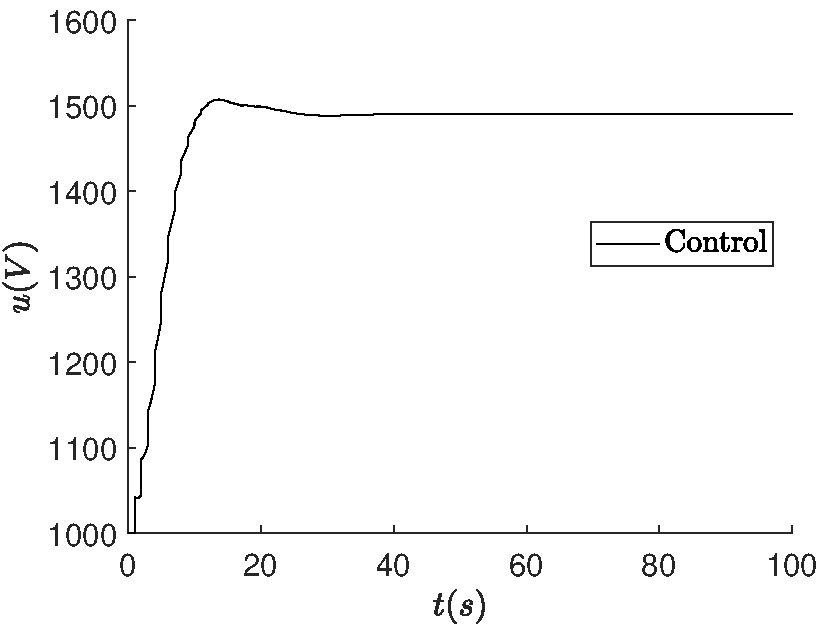
\includegraphics[scale=0.425]{files/feedback/Ref!0/control_sfc_u_1_5_ref_dif_0.pdf}
            \caption{Control action.}
        \end{subfigure}
        \vskip0.1cm
        \begin{subfigure}[b]{0.475\textwidth}   
            \centering 
            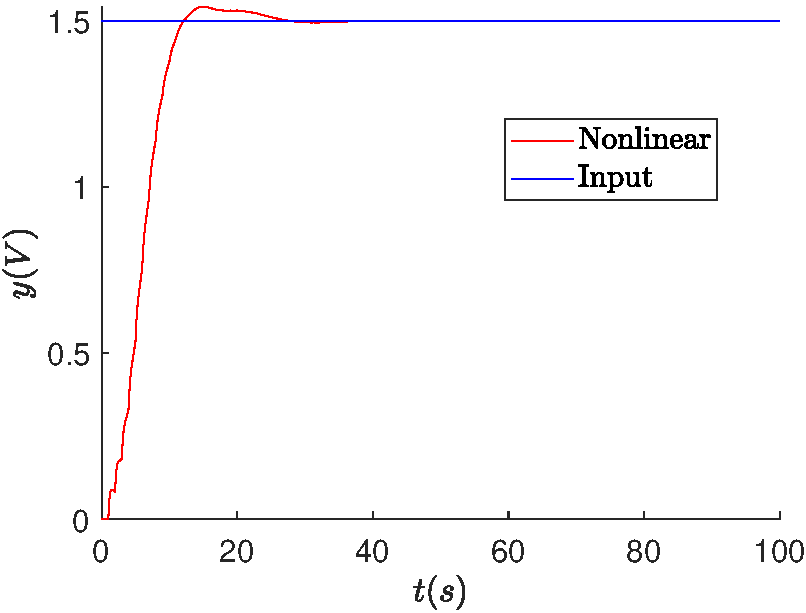
\includegraphics[scale=0.425]{files/feedback/Ref!0/sfc_u_1_5_ref_dif_0.pdf}
            \caption{Output.}
        \end{subfigure}
        \caption{Rössler system simulation with discrete state feedback controller $r(t)=1.5$.}
        \label{fig:feedback_u_1_5}
	\end{figure}
	
	Finally, one last constant reference was simulated: $r(t)=-2$. As shown in Fig. \ref{fig:feedback_u_-2}, the controller manages to stabilize the system eliminating steady-state error but with high frequency oscillations.
	
	\begin{figure}
        \centering
        \begin{subfigure}[b]{0.475\textwidth}
            \centering
            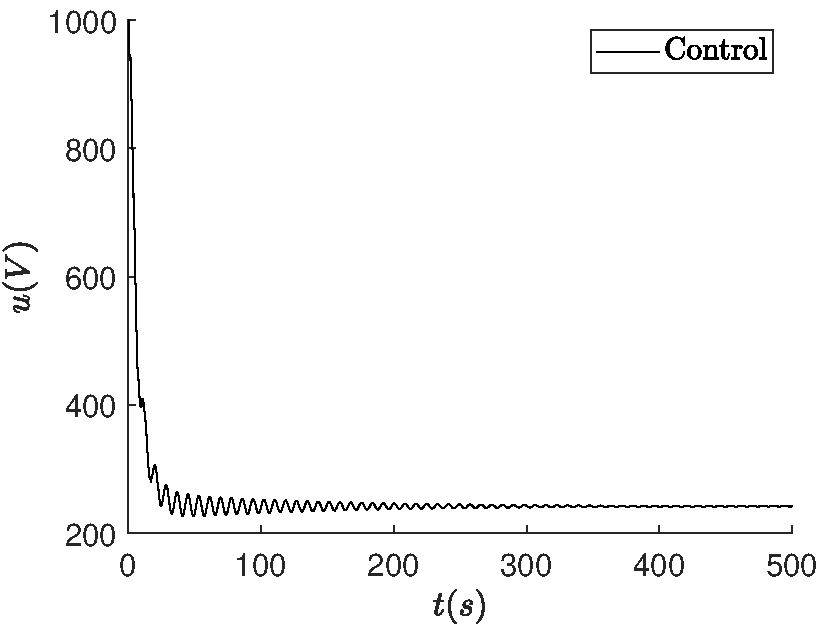
\includegraphics[scale=0.425]{files/feedback/Ref!0/control_sfc_u_-2_ref_dif_0.pdf}
            \caption{Control action.}
        \end{subfigure}
        \vskip0.1cm
        \begin{subfigure}[b]{0.475\textwidth}   
            \centering 
            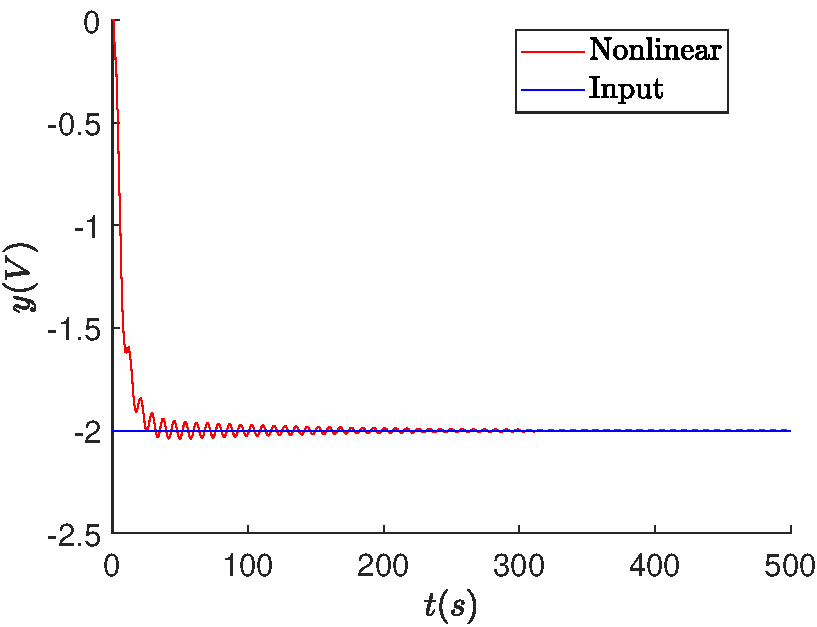
\includegraphics[scale=0.425]{files/feedback/Ref!0/sfc_u_-2_ref_dif_0.pdf}
            \caption{Output.}
        \end{subfigure}
        \caption{Rössler system simulation with discrete state feedback controller $r(t)=-2$.}
        \label{fig:feedback_u_-2}
	\end{figure}
	
	Next, a variable reference was tested, using $r(t)=0.01t$. The control action and the system's output is presented in \ref{fig:feedback_u_ramp_0_01}; notice that the steady-state for the Rössler system is parallel to the desired reference, this will be discussed in the next section.
	
	\begin{figure}
        \centering
        \begin{subfigure}[b]{0.475\textwidth}
            \centering
            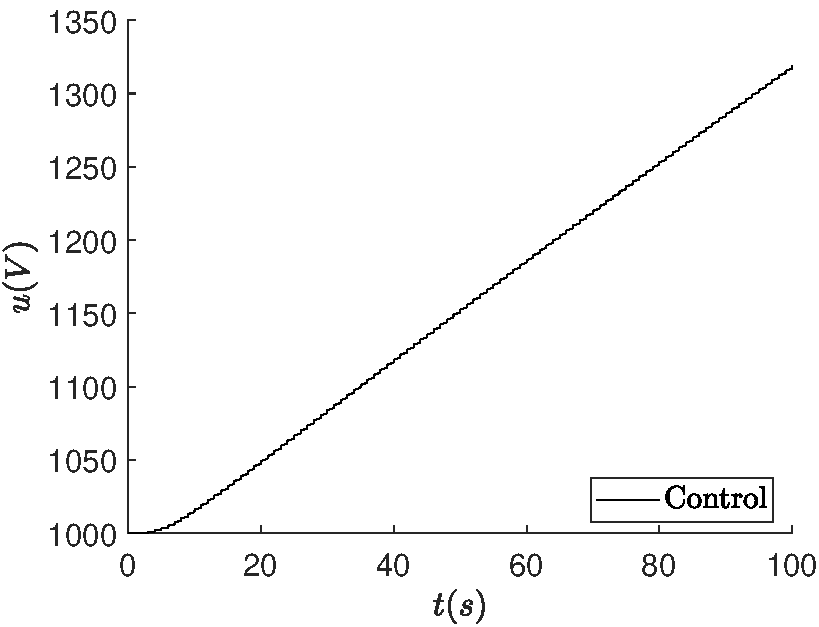
\includegraphics[scale=0.425]{files/feedback/Ref!0/control_sfc_ramp_0_01_ref_dif_0.pdf}
            \caption{Control action.}
        \end{subfigure}
        \vskip0.1cm
        \begin{subfigure}[b]{0.475\textwidth}   
            \centering 
            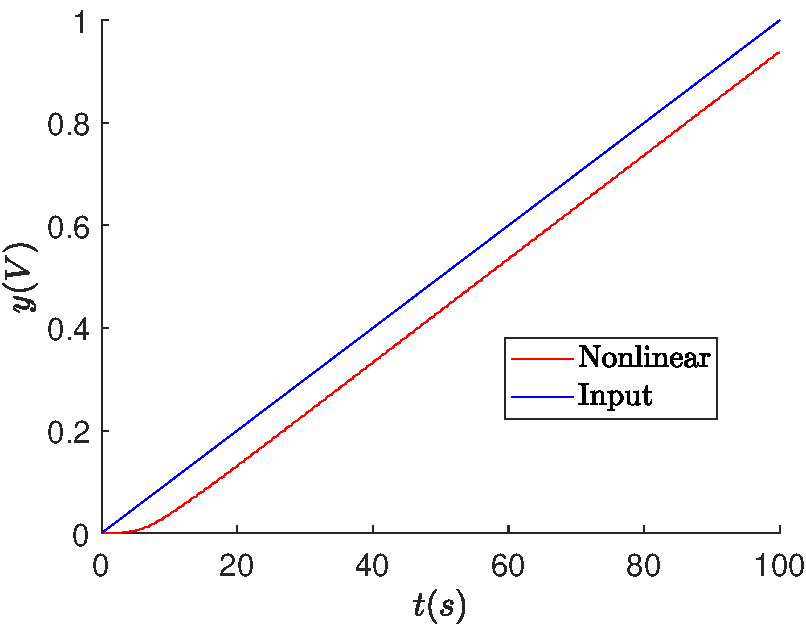
\includegraphics[scale=0.425]{files/feedback/Ref!0/sfc_ramp_0_01_ref_dif_0.pdf}
            \caption{Output.}
        \end{subfigure}
        \caption{Rössler system simulation with discrete state feedback controller $r(t)=-2$.}
        \label{fig:feedback_u_ramp_0_01}
	\end{figure}
	
\subsection{Uncertainty Analysis}
The uncertainty analysis was performed for the analytic discrete PID controller, for the state feedback controller with and without steady-state error. Applying the procedure described in section \ref{sec:uncertainty}, the parameter $R_a=500k\Omega$ will be first changed by $10\%$ (upwards and downwards) and then some other important values will be selected. The following simulations are set for $r(t)=1$.

For the analytic discrete PID controller, the first two simulations are for changing $R_a$ by $10\%$ upwards ($550k\Omega$) and downwards ($450k\Omega$). In Figs. \ref{fig:sens_ra_550}-\ref{fig:sens_ra_450}, these simulations are presented, notice that this controller works properly for these changes in $R_a$.

    \begin{figure}
        \centering
        \begin{subfigure}[b]{0.475\textwidth}
            \centering
            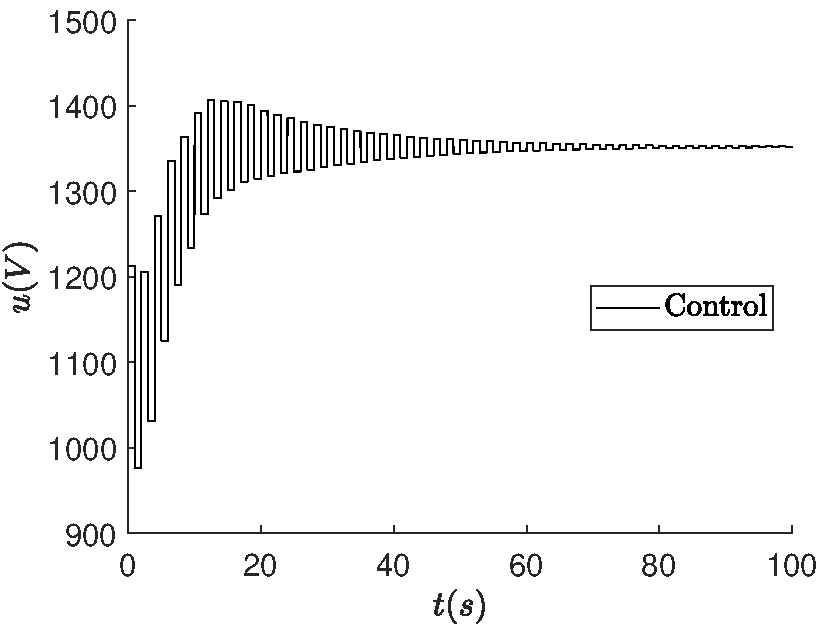
\includegraphics[scale=0.425]{files/sens_analysis/PID/control_analytic_a_550.pdf}
            \caption{Control action.}
        \end{subfigure}
        \vskip0.1cm
        \begin{subfigure}[b]{0.475\textwidth}   
            \centering 
            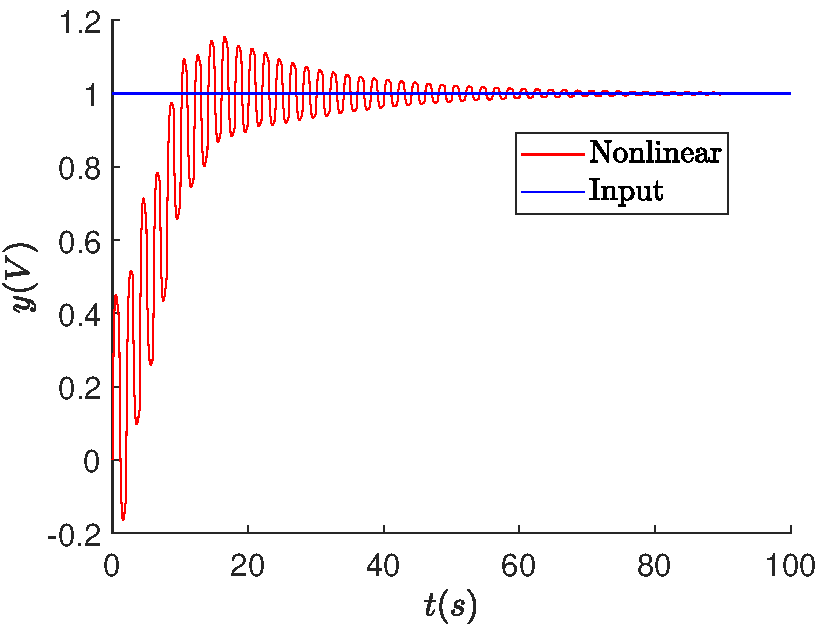
\includegraphics[scale=0.425]{files/sens_analysis/PID/analytic_sensitivity_a_550.pdf}
            \caption{Output.}
        \end{subfigure}
        \caption{Analytic discrete PID controller for $R_a=550k\Omega$.}
        \label{fig:sens_ra_550}
	\end{figure}
	
	\begin{figure}
        \centering
        \begin{subfigure}[b]{0.475\textwidth}
            \centering
            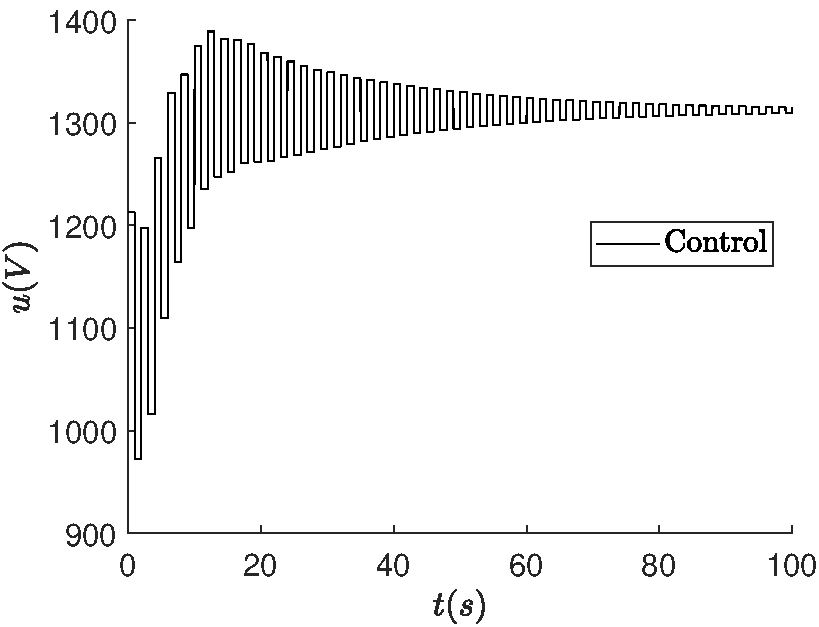
\includegraphics[scale=0.425]{files/sens_analysis/PID/control_analytic_a_450.pdf}
            \caption{Control action.}
        \end{subfigure}
        \vskip0.1cm
        \begin{subfigure}[b]{0.475\textwidth}   
            \centering 
            \includegraphics[scale=0.425]{files/sens_analysis/PID/analytic_sensitivity_a_450.pdf}
            \caption{Output.}
        \end{subfigure}
        \caption{Analytic discrete PID controller for $R_a=450k\Omega$.}
        \label{fig:sens_ra_450}
	\end{figure}
	
	Next, a larger change upwards in $R_a$ was performed: $R_a=2500k\Omega$. In Fig. \ref{fig:sens_ra_2500} the results for the controller and the output are presented, note that the system achieves stability and steady-state error elimination with smaller overshoot than the previous simulations; but the control action is on the limit, as it is about to reach its maximum value.
	
	\begin{figure}
        \centering
        \begin{subfigure}[b]{0.475\textwidth}
            \centering
            \includegraphics[scale=0.425]{files/sens_analysis/PID/control_analytic_a_2500.pdf}
            \caption{Control action.}
        \end{subfigure}
        \vskip0.1cm
        \begin{subfigure}[b]{0.475\textwidth}   
            \centering 
            \includegraphics[scale=0.425]{files/sens_analysis/PID/analytic_sensitivity_a_2500.pdf}
            \caption{Output.}
        \end{subfigure}
        \caption{Analytic discrete PID controller for $R_a=2500k\Omega$.}
        \label{fig:sens_ra_2500}
	\end{figure}
	
	Finally, a larger change downwards was performed $R_a=300k\Omega$. Fig. \ref{fig:sens_ra_300} shows the results for this simulation. Notice that the system is critically stable around $y(t)=1V$, this implies that the controller is on the edge of making the system unstable and it cannot eliminate steady-steady error. Note that the control signal is almost saturated.
	\begin{figure}
        \centering
        \begin{subfigure}[b]{0.475\textwidth}
            \centering
            \includegraphics[scale=0.425]{files/sens_analysis/PID/control_analytic_a_300.pdf}
            \caption{Control action.}
        \end{subfigure}
        \vskip0.1cm
        \begin{subfigure}[b]{0.475\textwidth}   
            \centering 
            \includegraphics[scale=0.425]{files/sens_analysis/PID/analytic_sensitivity_a_300.pdf}
            \caption{Output.}
        \end{subfigure}
        \caption{Analytic discrete PID controller for $R_a=300k\Omega$.}
        \label{fig:sens_ra_300}
	\end{figure}
	
	For the discrete state feedback controller, the same procedure was attempted. The parameter $R_a$ was changed to $550k\Omega$ and $450k\Omega$. Figs. \ref{fig:sens_ra_550_state}-\ref{fig:sens_ra_450_state} show both simulations (recall that $r(t)=0$ in these controllers), where it can be observed that these controller does not work properly (they do not stabilize in the reference).
	
	\begin{figure}
        \centering
        \begin{subfigure}[b]{0.475\textwidth}
            \centering
            \includegraphics[scale=0.425]{files/sens_analysis/Ref0/control_analysis_sfc_a_550.pdf}
            \caption{Control action.}
        \end{subfigure}
        \vskip0.1cm
        \begin{subfigure}[b]{0.475\textwidth}   
            \centering 
            \includegraphics[scale=0.425]{files/sens_analysis/Ref0/analysis_sfc_a_550.pdf}            \caption{Output.}
        \end{subfigure}
        \caption{Discrete state feedback controller controller for $R_a=550k\Omega$.}
        \label{fig:sens_ra_550_state}
	\end{figure}
	
	\begin{figure}
        \centering
        \begin{subfigure}[b]{0.475\textwidth}
            \centering
            \includegraphics[scale=0.425]{files/sens_analysis/Ref0/control_analysis_sfc_a_450.pdf}
            \caption{Control action.}
        \end{subfigure}
        \vskip0.1cm
        \begin{subfigure}[b]{0.475\textwidth}   
            \centering 
            \includegraphics[scale=0.425]{files/sens_analysis/Ref0/analysis_sfc_a_450.pdf}
            \caption{Output.}
        \end{subfigure}
        \caption{Discrete state feedback controller controller for $R_a=450k\Omega$.}
        \label{fig:sens_ra_450_state}
	\end{figure}
	
	Finally, the discrete state feedback controller with no steady-state error was analyzed with the same parameters as the discrete analytical PID controller. Thus, the first two simulations are for $R_a=550k\Omega$ and $R_a=450k\Omega$, displayed in Figs. \ref{fig:sens_ra_550_state_noess}-\ref{fig:sens_ra_450_state_noess}, as it can be seen, the controller works properly for both changes, showing no steady-state error and good behavior (no significant overshoot or oscillation).
	
	\begin{figure}
        \centering
        \begin{subfigure}[b]{0.475\textwidth}
            \centering
            \includegraphics[scale=0.425]{files/sens_analysis/Ref!0/control_analysis_sfc_a_550_ref_dif_0.pdf}
            \caption{Control action.}
        \end{subfigure}
        \vskip0.1cm
        \begin{subfigure}[b]{0.475\textwidth}   
            \centering 
            \includegraphics[scale=0.425]{files/sens_analysis/Ref!0/analysis_sfc_a_550_ref_dif_0.pdf}            \caption{Output.}
        \end{subfigure}
        \caption{Discrete state feedback controller ($r(t)\neq0$) controller for $R_a=550k\Omega$.}
        \label{fig:sens_ra_550_state_noess}
	\end{figure}
	
	\begin{figure}
        \centering
        \begin{subfigure}[b]{0.475\textwidth}
            \centering
            \includegraphics[scale=0.425]{files/sens_analysis/Ref!0/control_analysis_sfc_a_450_ref_dif_0.pdf}
            \caption{Control action.}
        \end{subfigure}
        \vskip0.1cm
        \begin{subfigure}[b]{0.475\textwidth}   
            \centering 
            \includegraphics[scale=0.425]{files/sens_analysis/Ref!0/analysis_sfc_a_450_ref_dif_0.pdf}
            \caption{Output.}
        \end{subfigure}
        \caption{Discrete state feedback controller ($r(t)\neq0$) controller for $R_a=450k\Omega$.}
        \label{fig:sens_ra_450_state_noess}
	\end{figure}
	
    Now, the same simulation was executed for $R_a=3000k\omega$ and the control signal and output can be observed in Fig. \ref{fig:sens_ra_3000_state_noess}. Notice that the control signal is almost saturated but the controller works perfectly, without overshoot relatively fast stabilization.
    \begin{figure}
        \centering
        \begin{subfigure}[b]{0.475\textwidth}
            \centering
            \includegraphics[scale=0.425]{files/sens_analysis/Ref!0/control_analysis_sfc_a_3000_ref_dif_0.pdf}
            \caption{Control action.}
        \end{subfigure}
        \vskip0.1cm
        \begin{subfigure}[b]{0.475\textwidth}   
            \centering 
            \includegraphics[scale=0.425]{files/sens_analysis/Ref!0/analysis_sfc_a_3000_ref_dif_0.pdf}
            \caption{Output.}
        \end{subfigure}
        \caption{Discrete state feedback controller ($r(t)\neq0$) controller for $R_a=3000k\Omega$.}
        \label{fig:sens_ra_3000_state_noess}
	\end{figure}
	
	Lastly, the parameter $R_a$ was set to $250k\Omega$ and the simulation was conducted one last time. These results are presented in Fig. \ref{fig:sens_ra_250_state_noess}; this simulation show that the controller cannot work properly, since the system reaches a critically-stable state, showing undesired steady-state error (although the control signal is not saturated).
	
	\begin{figure}
        \centering
        \begin{subfigure}[b]{0.475\textwidth}
            \centering
            \includegraphics[scale=0.425]{files/sens_analysis/Ref!0/control_analysis_sfc_a_250_ref_dif_0.pdf}
            \caption{Control action.}
        \end{subfigure}
        \vskip0.1cm
        \begin{subfigure}[b]{0.475\textwidth}   
            \centering 
            \includegraphics[scale=0.425]{files/sens_analysis/Ref!0/analysis_sfc_a_250_ref_dif_0.pdf}
            \caption{Output.}
        \end{subfigure}
        \caption{Discrete state feedback controller ($r(t)\neq0$) controller for $R_a=250k\Omega$.}
        \label{fig:sens_ra_250_state_noess}
	\end{figure}